\documentclass[10pt,twocolumn,letterpaper]{article}

% ຂອງຂ້ອຍເອງ
\usepackage{booktabs}
% \usepackage{caption}
% \captionsetup[table]{skip=8pt}   % ສົມພັດກັບຕາຕະລາງເທົ່ານັ້ນ
\usepackage{stfloats}  % ເພີ່ມນີ້ເຂົ້າໄປໃນ preamble
\usepackage{float}
\usepackage[T1]{fontenc}

% \usepackage{fontspec}
\usepackage[english]{babel}

% load Lao via babelprovide, turn on "onchar=ids" for automatic shaping
\babelprovide[import,onchar=ids fonts]{lao}

% main (rm) font for Latin
\babelfont{rm}{Noto Serif}

% Lao text in Noto Serif Lao at 1.2× scale
\babelfont[lao]{rm}{Noto Serif Lao}
\babelfont[lao]{sf}{Noto Serif Lao}

% alternate (sans-serif) font for Latin
\babelfont{alt}{Lato}

% Lao text in Noto Serif Lao for the alt family too
\babelfont[lao]{alt}{Noto Serif Lao}

% GPT: LuaTeX doesn’t have built-in Lao line-breaking rules, but babel can assimilate line breaks to hyphenation if you supply some simple “patterns” for common syllable boundaries. Add this to your preamble:
\babelpatterns[lao]{%
  1ດ 1ມ 1ອ 1ງ 1ກ 1າ 1ັ 1ິ 1ີ 1້ 1ົ 1ູ%
}

\usepackage{cvpr}
\usepackage{times}
\usepackage{epsfig}
\usepackage{graphicx}
\usepackage{amsmath}
\usepackage{amssymb}


\usepackage[breaklinks=true,bookmarks=false]{hyperref}
\cvprfinalcopy % *** ເດີນສາຍນີ້ສຳລັບການສົ່ງຂັ້ນສຸດທ້າຍ

\makeatletter
\def\cvprsubsection{\@startsection {subsection}{2}{\z@}
    {8pt plus 2pt minus 2pt}{6pt}{\bfseries\normalsize}}
\makeatother

\def\cvprPaperID{****} % *** ໃສ່ລະຫັດ CVPR Paper ID ທີ່ນີ້
\def\httilde{\mbox{\tt\raisebox{-.5ex}{\symbol{126}}}}

% ໜ້າຖືກນັບໃນໂໝດສົ່ງ, ແລະບໍ່ນັບໃນສະບັບພ້ອມພິມ
%\ifcvprfinal\pagestyle{empty}\fi
\setcounter{page}{1}
\begin{document}

%%%%%%%%% TITLE
\title{ບົດນຳທີ່ຂັບເຄື່ອນດ້ວຍຂໍ້ມູນ ECDO ພາກ 1/2: ເຂົ້າໃຈປັດຈຸບັນຂອງທຶນນິຕິສາດການເດືອດຂອງ Core-Mantle ແບບບໍ່ສອດຄ່ອງ Dzhanibekov Oscillation (ECDO) ທີ່ຖືກເອີ້ນວ່າ “ແຜ່ນດິນໂລກກັບ”}

\author{Junho\\
ຕີພິມ ເດືອນກຸມພາ 2025\\
ເວັບໄຊ (ດາວໂຫຼດກະດານທີ່ນີ້): \href{https://sovrynn.github.io}{sovrynn.github.io}\\
ທີ່ເກັບງານຄົ້ນຄວ້າ ECDO: \href{https://github.com/sovrynn/ecdo}{github.com/sovrynn/ecdo}\\
{\tt\small junhobtc@proton.me}
}

\maketitle
%\thispagestyle{empty}

\begin{abstract}
ໃນເດືອນພຶດສະພາ 2024, ຜູ້ໃຊ້ອິນເຕີເນັດນິນທີ່ໃຊ້ນາມສຸດໃນຊື່ວ່າ “The Ethical Skeptic” \cite{0} ໄດ້ແບ່ງປັນທຶດສະດີໃໝ່ຂອງເຂົາທີ່ມີຊື່ວ່າ Exothermic Core-Mantle Decoupling Dzhanibekov Oscillation (ECDO) \cite{1}. ທຶດສະດີນີ້ແນະນຳວ່າ ໂລກໄດ້ເຄີຍປະສົບກັບການສຳຫຼວດແກນຫມຸນຂອງຕົນເອງຢ່າງກະທັນຫັນ ເພາະສາເຫດນີ້ເຮັດໃຫ້ເກີດນ້ຳຖ້ວມທົ່ວໂລກ ເມື່ອນ້ຳທະເລຫຼົ່ນລົງເຫນືອທະວີບແນວນອນຈາກຄວາມເສຍຫຍຸ້ນຂອງການຫມຸນ. ນອກນີ້ຍັງມີວິທີການອະທິບາຍທາງພູມສາດແລະຫຼັກຖານຂໍ້ມູນວ່າອາດຈະເກີດການຫມຸນກັບເຫມືອນນີ້ອີກໃນໄມ່ຊ້າ. ແມ່ນແມ່ນວ່າການຄາດຄະເນເກື່ອບຖຶງນ້ຳຖ້ວມຫຼືວັນສິ້ນໂລກນັ້ນບໍ່ໃຊ້ຂ່າວໃໝ່, ແຕ່ທຶດສະດີ ECDO ນີ້ມີຄວາມໜ້າສົນໃຈເປັນພິເສດເນື່ອງຈາກຫຼັກຖານທາງວິທະຍາສາດ, ສະໄໝໃໝ່, ຫຼາຍສາຂາ, ແລະອີງຂໍ້ມູນຈິງ.

ເອກະສານນີ້ເປັນສ່ວນທຳອິດຂອງສອງສ່ວນທີ່ສະຫຼຸບຫຍໍ້ພາຍໃນເວລາຫົກເດືອນຂອງການຄົ້ນຄວ້າອິດສະຫຼາດ \cite{2,20} ກ່ຽວກັບທຶດສະດີ ECDO. ໃນນີ້ ຂ້ອຍຂໍເນັ້ນສາມປະເດັນຫຼັກ:

\begin{flushleft}
\begin{enumerate}
    \item ພົບຫຼັກຖານວ່າການຫມຸນກັບແນວ “Earth flip” ແບບ ECDO ເກີດຂຶ້ນຫຼາຍຄັ້ງໃນປະຫວັດສາດສະໄໝໃກ້ນີ້ຂອງມວນມະນຸດ, ເຫັນໄດ້ຈາກນິທານນ້ຳຖ້ວມແລະຫຼັກຖານທາງພູມສາດທີ່ບົດສະແດງການນ້ຳຖ້ວມທົ່ວທະວີບ.
    \item ທິດທາງແລະຂະຫນາດປະມານຂອງການຫມຸນກັບແນວ “Earth flip” ໃນອະດີດສາມາດຄຳນວນໄດ້.
    \item ຂໍ້ມູນລ່າສຸດທາງພູມເຫມາແລະພູມສາດບົດສະແດງວ່າການຫມຸນກັບໃຫມ່ອາດຈະເກີດຂຶ້ນໄດ້ ແລະການປ່ຽນແປງສະພາບອາກາດອາດມີສາເຫດມາຈາກການປ່ຽນແປງຄິດຖຶງຢູ່ໃນໂລກ ແທນທີ່ຈະເປັນສາຫຼັກມາຈາກມະນຸດ.
\end{enumerate}
\end{flushleft}

ນອກນີ້, ຂ້ອຍຍັງອະທິບາຍກ່ຽວກັບຟິສິກທີ່ເປັນສາເຫດຂອງການ “Earth flip” ທີ່ຖືກສະເໜີໂດຍທຶດສະດີ ECDO.

ໃນເອກະສານນີ້, ຂ້ອຍພະຍາຍາມຢູ່ໃນມຸມມອງທີ່ເປັນກາງ ໂດຍເນັ້ນໃສ່ຂໍ້ມູນທີ່ຫນັກແນ່ນ, ລະຫັດກຸ່ມສ່ວນທີ່ດຶງດູດແຕ່ດາວແປດ ແລະເນັ້ນຍ້ຳວ່ານີ້ແມ່ນຫົວຂໍຫຼັກທີ່ມະນຸດມີຄວາມຈຳເປັນເຮັດການສຶກສາຕໍ່ໄປ.
\end{abstract}
\section{ການນໍາໃຊ້}

ເຣື່ອງລາວກ່ຽວກັບນ້ຳຖ້ວມໃຫຍ່ບໍ່ແມ່ນເລື່ອງໃໝ່ - ແທ້ຈິງແລ້ວ, ມັນພົບເຫັນໃນທຸກວັດທະນະທໍາໃຫຍ່ທົ່ວໂລກ, ກວ້າງຂວາງທຸກບໍ່ອູ່ທີ່ເກີດອາລະຍະທຳ. ການວາດຮູບ (ຮູບທີ່ \ref{fig:1}) ການປະກອບກັນຂອງເລື່ອງນ້ຳຖ້ວມ 267 ເລື່ອງ \cite{3} ເຫັນວ່າເກືອບທຸກບໍ່ອູ່ທີ່ຢູ່ອາໄສຂອງໂລກມີເລື່ອງນ້ຳຖ້ວມ.

\begin{figure}[h]
\begin{center}
% \fbox{\rule{0pt}{2in} \rule{0.9\linewidth}{0pt}}
   \includegraphics[width=1\linewidth]{b.png}
\end{center}
   \caption{ສະຖານທີ່ຂອງເລື່ອງນ້ຳຖ້ວມທົ່ວໂລກ \cite{3}.}
\label{fig:1}
\label{fig:onecol}
\end{figure}

ການສັງເກດເບິ່ງເລື່ອງນ້ຳຖ້ວມເຫຼົ່ານີ້ ສະແດງໃຫ້ເຫັນວ່າ ນີ້ບໍ່ແມ່ນນ້ຳຖ້ວມທົ່ວໄປ, ແຕ່ເປັນພິບັດທີ່ທຳລາຍທຸກຢ່າງ ແລະມີນ້ຳຖ້ວມຫຼາຍປະສານກັນທີ່ກວາດລ້າງທະວິບໃຫຍ່ໃຫ້ສະອາດ.

\subsection{ເລື່ອງເກົາຫຼິມພິບັດຂອງຊາວພື້ນເມືອງອາເມລິກາ}

ເລື່ອງລາວຂອງຊາວພື້ນເມືອງອາເມລິກາ ເປັນເລື່ອງລາວທີ່ມີຄວາມສົດຈິງກ່ຽວກັບພິບັດງານໃຫຍ່ຂອງໂລກ. ຊົນເຜົ່າ Hopi, ຊາວພື້ນເມືອງທີ່ອາໄສຢູ່ພາກຕາເຫນືອຂອງລັດ Arizona, ເວົ້າວ່າ, \textit{"..Sótuknang ເອີ້ນໃຫ້ບັນດາມົດໄມ້ເປີດໂລກໃຕ້ດິນຂອງພວກເຂົາສໍາລັບບຸກຄົນທີ່ຖືກເລືອກ. ເມື່ອພວກເຂົາຢູ່ໃຕ້ດິນຢ່າງປອດໄພ, Sótuknang ສັ່ງໃຫ້ຝາແຝດ, Pöqánghoya ແລະ Palöngawhoya, ອອກຈາກຕຳແໜ່ງທີ່ທາງເໜືອແລະທາງໃຕ້ຂອງແກນໂລກ, ທີ່ພວກເຂົາຖືກຕັ້ງໄວ້ເພື່ອຮັກສາໃຫ້ໂລກຫັນຕົວໄດ້ຢ່າງຖືກຕ້ອງ. \textbf{ຝາແຝດເພິ່ງຈະລະຕຳແໜ່ງຂອງພວກເຂົາ ເມື່ອໂລກ, ໂດຍເປົ້າໝາຍບໍ່ມີໃຜຄວບຄຸມ, ກະທົບດຸຫລູດຫວັ່ນ, ໝຸນຕົວໄປຢ່າງຜິດປົກກະຕິ, ແລ້ວມັນກໍ່ລ້ມສອງຄັ້ງ.} ພູເຂົາດ່ຳຕົວລົງໃນທະເລກັບສຽງນ້ຳດັງສະຫຼຸບ, ທະເລແລະທະເລສາບໄຫວ່ນເຫື້ອນເຫນືອບົດແຜ່ນດິນ; ແລະເມື່ອໂລກຫມຸນຕົວໄປໃນອາກາດໜາວແລະບໍ່ມີຊີວິດມັນກໍ່ກາຍເປັນນຳ້ແຂງ"} \cite{4}.
หลายໆເລື່ອງລາວເຫຼົ່ານີ້ອະທິບາຍຢ່າງຖືກຕ້ອງເຖິງຂະໜາດອັນມະຫຼານຂອງນໍ້າຖ້ວມ, ບັນຍາຍວ່າມະຫາສຸມທະເລໄດ້ເພີ່ມຂື້ນຈົນຈົບເຫຼືອເພີຍແຕ່ຍອດພູສູງທີ່ສຸດ. ຊາວສະໂກໂຄມິດທີ່ອາໄສຢູ່ລັດວໍຊິງຕັນ, ໄດ້ເວົ້າວ່າ, \textit{"ພຣະວິນຍານອັນຫຼວງເອົາໃຈເກີດຄວາມໂກດຕໍ່ການຊົ່ວຮ້າຍຂອງຜູ້ຄົນແລະສັດ, ຈຶ່ງຕັດສິນໃຈກຳຈັດໂລກໃຫ້ເຫຼືອເພີຍແຕ່ສັດດີ, ຄົນດີຄົນໜຶ່ງ ແລະຄອບຄົວຂອງເຂົາ. ຕາມຄຳສັ່ງຂອງພຣະວິນຍານອັນຫຼວງ, ຜູ້ຊາຍນັ້ນຍິງລູກດອກໄປໃສ່ເມກ, ແລ້ວຍິງລູກຕໍ່່ໄປໃສ່ລູກນັ້ນ, ຢ່າງນີ້ໄປເຮັດເຊືອກດອກລູກສອນຈາກເມກລົງສູ່ພື້ນ. ສັດດີແລະຄົນດີໄດ້ປີນຂື້ນໄປ. ສັດຊົ່ວແລະງູເລີ່ມປີນຂື້ນໃສ່ເຊືອກ, ແຕ່ຜູ້ຊາຍນັ້ນບິດເຊືອກອອກ. \textbf{ແລ້ວພຣະວິນຍານອັນຫຼວງໄດ້ເຮັດໃຫ້ຝົນຕົກຫຼາຍມື້, ນໍ້າຖ້ວມຈົນເຖິງຂອບຫິມະຂອງທາຄົມາ (ພູຣາເນຍ)}. ຫລັງຈາກຄົນແລະສັດຊົ່ວທັງໝົດຈົນນໍ້າ, ພຣະວິນຍານຫຼວງກໍ່ຢຸດຝົນ, ນໍ້າຄ່ອຍໆຫຼົງລົງ, ແລະຄົນດີ ແລະສັດດີກໍ່ປີນລົງ"} \cite{3}. ເພື່ອເປັນການອ້າງອີງ, ພູຣາເນຍແມ່ນພູໄຟປົວແຫ່ງຫນຶ່ງໃນລັດວໍຊິງຕັນ ມີຄວາມສູງສຸດ 4392.5 ແມັດເ໫ືອດລະດັບນໍ້າທະເລ.

ເລື່ອງນໍ້າຖ້ວມຈາກຊາວ Makah ຢູ່ລັດວໍຊິງຕັນໄດ້ກ່າວເຖິງນໍ້າຖ້ວມຫຼາຍຂັ້ນຕອນຂອງນໍ້າ "ອຸ່ນໆ", ໃຫ້ເຫັນວ່ານີ້ບໍ່ແມ່ນນໍ້າຖ້ວມທົ່ວໄປ: \textit{"ທະເລຍົກສູງຂຶ້ນຈົນຕັດສັນຕິເຫຼົາຄົບ. ແລ້ວນໍ້ານັ້ນຖອນລົງ, ເຖິງຈຸດຕ່ຳສຸດຫຼັງຈາກສີ່ມື້, ປ່ອຍ Neah Bay ໃຫ້ສູງແລະແຫ້ງ. ແລ້ວນໍ້າກໍ່ຢືນສູງເພີ່ມເທິງເຫຼືອຍອດພູ. \textbf{ນໍ້າທີ່ຂື້ນມານັ້ນອຸ່ນຫຼາຍ.} ຄົນທີ່ມີເຮືອໄດ້ຂົນເຄື່ອງຂອງພວກເຂົາແລະຖືກພາໄປເທິງເໜືອໄກ. ຫຼາຍຄົນເສຍຊີວິດເມື່ອເຮືອພວກເຂົາຕິດໃນຕົ້ນໄມ້. ທະເລກັບຄືນປົກກະຕິຫຼັງຈາກອີກສີ່ວັນ, ແລະຄົນເຫຼົ່ານັ້ນພົບຕົນເອງຢູ່ເທິງເໜືອ ເພື່ອນຍາດພວກເຂົາອາໄສຢູ່ທີ່ນັ້ນຈົນຖຶງປັດຈຸບັນ"} \cite{3}.

\subsection{ເລື່ອງລາວພິຍະຕິບັດຈາກຈີນ}

ອີກຝັ່ງຫນຶ່ງຂອງມະຫາສຸມທະເລບໍກ່ອນ, ອານາຈັກຈີນສະເຫີນລ້ານກ່ອນເກີດຜູ້ລົງຂອງນໍ້າຖ້ວມ. ລາຊະວົງຊຽດິນາສະ, ຖືກຄາດຄະເນວ່າຈະມີຢູ່ປະມານ 2000 ກ່ອນຄຣິດການ, ເກີດຂຶ້ນໂດຍພະຍູອຸຍິງຫຼວງ, ຜູ້ຢຸດນໍ້າຖ້ວມອັນໃຫຍ່ຂອງກຸນ-ຢູ \cite{6}. ໃນເວລານັ້ນ, \textit{"... ເຫດອັດສະຈັນໄດ້ເກີດຂຶ້ນວ່າຕາວັນໃນໄລຍະສິບມື້ບໍ່ຕົກ, ປ່າໄດ້ສັນຕິການເຜົາໄຫ້, ແລະມີແມງສົ້ມອັນຊົ່ວຮ້າຍເກີດຂຶ້ນໄດ້... ຄືນແຫ່ງການອາບນໍ້າອັນໃຫຍ່"ທີ່ເຖິງຟ້າ"ຣ່ວງຫຼົງສູ່ດິນຈີນ. \textbf{"ນໍ້າຢູ່ສູງໆໃນພູສູງ, ແລະພູຕໍາໆບໍ່ເຫັນເລີຍ"}... "ອັນຕະລາຍໃນທີ່ນໍ້າທ່ວມ", ຈັກກະພັດໄດ້ກ່າວ. "ໃນຂະໜາດກວ້າງຂອງມັນ, ມັນຄອບຄຸມຫຼວງຊື້ນຶ່ງແລະຢ້ານຢ້ານໃນຄວາມສູງໃຫຍ່, ຄືເປັນອັນອັນຕະລາຍໃຫ້ເຖິງຟ້າ." ຈັກກະພັດສັ່ງໃຫ້ພະຍາຍາມເປີດທາງໃຫ້ນໍ້າທີ່ຕິດຢູ່ໃນເພີ່ນຂອງພູ. ຫຼາຍປີທີ່ປະຊາກອນໂຮມແຮງງານ, ພະຍາຍາມປົດປ່ອຍພື້ນພະນາແລະເພີ່ນເພື່ອປົດນໍ້າໂດຍການຂຸດຄໍາແລະລະບາຍນໍ້າອອກ. ນານປີທີ່ພະຍາຍາມທັງໝົດເກີນປະໂຫຍດ. ລັດທີ່ຮັບຜິດຊອບວຽກອັນສໍາຄັນແລະຫຼາຍຫຼາຍນີ້, ຄວານ, ຖືກຕັດສິນໂທດປາງຊີວິດເພາະຫາການລົ້ມເຫລວ... ແລະມີແຕ່ລູກຂອງເຂົາ ຢູ, ຈຶ່ງສາມາດເຮັດໃຫ້ດິນໄພ. ຄວາມສໍາເລັດນີ້ໄດ້ຖືກຍົກຫຼວງຈົນຢູໄດ້ເປັນຈັກກະພັດຈີນຫຼັງຈາກກົງຊຸນ, ຜູ້ສືບຕໍ່ຄົນທຳອິດຂອງຢາໂຫວ"} \cite{5}.

ເບິ່ງເຫັນວ່າບໍ່ພຽງແຕ່ຈີນຖືກນໍ້າຖ້ວມ, ແຕ່ຍັງມີຄວາມຈໍາເປັນທີ່ຈະວັດທິດທາງອີກເທື່ອ ແລະການເຄື່ອນໄຫວຂອງຕາເວັນ ແລະດວງຈັນ, ເຊິ່ງບໍລິບາຍວ່າການຫມຸນຂອງໂລກອາດຈະໄດ້ປ່ຽນໄປໃນໄລຍະນໍ້າຖ້ວມ: \textit{\textbf{"ຈັກກະພັດນີ້ສົ່ງນັກວິຊາການໄປທີ່ຕ່າງໆໃນຈີນ ແລະແມ່ນກະທັ່ງໄປອິນໂດຈີນ ເພື່ອຊອກຫາຕຳແໜ່ງຫນືອ, ໃຕ້, ຕາເວັນອອກ ແລະຕາເວັນຕົກໂດຍສັງເກດທິດທາງຕາເວັນຂຶ້ນ ແລະຕົກ ແລະການເຄື່ອນໄຫວຂອງດາວ.} ເຂົາຍັງໃຫ້ຂະເໝານວ່ານັກດາວສາທົບ ຄົ້ນຫາໄລຍະເວລາຂອງ຤ູກິດ ແລະຕັ້ງປົກກະຕິເກັບປິດໃໝ່... "ດັ່ງນັ້ນຢາໂຫວ [ຢາໂຫວ] ໄດ້ສັ່ງເຮົາ ແລະໂຮ, ຢ່າງເຄົາລົບຕໍ່ເຈົ້າຟ້າກວ້າງຂວາງ, ຄໍານວນແລະແຕ້ມໄວ້ການເຄື່ອນໄຫວ ແລະການປະກົດຂອງຕາເວັນ, ດວງຈັນ, ດາວ ແລະພຶດສະຈັກ; ແລະຕັ້ງໃຫ້ຮູ້ລະດູການໃໝ່ແກ່ປະຊາຊົນ""} \cite{5}.

ບັນທຶກເຫດການພິຍະຕິບັດໃນປະຫວັດສາດຈີນ ແທ້ໆແລ້ວໄດ້ຍ້ອນໄປກ່ອນລາຊະວົງຊຽດິນາສະ, ໄປຮອດສະໄໝສາມກະສັດແລະຫ້າຈັກກະພັດ \cite{7}. ຫນູວາ, ໜຶ່ງໃນສາມກະສັດ ແລະເປັນທີ່ສຳຄັນໃນເລື່ອງສ້າງໂລກຂອງຈີນ, ໄດ້ກັ້ນນໍ້າຖ້ວມໃນຍາມທີ່ເກີດຫຍຸງໃຫຍ່ ແລະຕຳແໜ່ງຮູບແບບການຫມຸນຂອງໂລກໄດ້ປ່ຽນໄປ: \textit{"ມີການຂັດຍ້ອງລະຫວ່າງພຣະອົງທີ່ມີອຳນາດສອງອົງ ແລະໃນທີ່ສຸດໄດ້ຕັດສິນໃຈສູ້ກັນ. ເມື່ອພຣະນໍ້າ Gong Gong ເຫັນວ່າຂ້ອຍຈະແພ້, ເຂົາເຊິ່ງຫົວເຂົາໄປກະແທກພູ Buzhou, ເສົາທີ່ຖືກຟ້າຂຶ້ນ. \textbf{ເສົານັ້ນພັງແລະເຮັດໃຫ້ຟ້າເອົາຫົວໄປທາງຕາເວັນຕົກ ແລະດິນເລື້ອນລົງໄປທາງຕາເວັນອອກໃຕ້.} ນັ້ນເຮັດໃຫ້ເກີດຄວາມພິຍະຕິບັດໃຫຍ່ໆ, ເຊັ່ນ ໄຟໃຫ້ບໍ່ຢຸດ, ນໍ້າຖ້ວມໃຫຍ່ໆ, ແລະສັດປ່າດຸຮ້າຍປາກົດ. ຫນູວາຕັດຂາເຕົ່າຍັກລົງແລະໃຊ້ມັນປົງເສົາທີ່ພັງ, ເບຍບາງສະພາບ ແລະປິດຟ້າທີ່ແຕກໂດຍຫີນສີທີ່ແຕກຕ່າງໆ, ແຕ່ເຘັ້ຍບໍ່ສາມາດແກ້ໄຂຟ້າເອົາຫົວໄດ້ເຕັມທີ່"} \cite{8}.

\subsection{ເລື່ອງລາວພິຍະຕິບັດໃນຍຸໂຣບ, ມາຍາ, ຕາເວັນອອກກາງ, ແລະອາຊຽນເຫນືອ}

ເນື່ອງຈາກມີເລື່ອງລາວພິຍະຕິບັດຫຼາຍເກີນຈະກ່າວໃນເອກະສານນີ້, ຂ້າພະເຈົ້າຂອບໃຈກ່າວເຖິງນິຍາຍຍໍ້ບາງສ່ວນຂອງວັດທະນະທຳອື່ນໆທີ່ມີເລື່ອງນີ້. ວັນນະຄະດີຢູໂຣບປະກອບມີນິຍາຍນໍ້າຖ້ວມສຳຄັນສາມເລື່ອງ, ແມ່ນຂອງ Deucalion, Ogyges, ແລະ Dardanus \cite{9,10}. ໃນເລື່ອງ Deucalion, \textit{"ຜ່ານເກົ້າມື້ຂອງນໍ້າຖ້ວມ, ໂລກຖືກທຳລາຍ ແລະຮຽນທ່າເຮືອຈອດຢູ່ຢອດພູ Parnassus"} ທີ່ມີຄວາມສູງສຸດ 2,457 ແມັດ \cite{11}. ວັນນະຄະດີມາຍາເຊື່ອວ່າເຄີຍມີພວກຕາເວັນສີ່ອາຍຸກ່ອນຕາວັນປະຈຸບັນ ແລະໄວ້ວ່າສະໄໝຕາເວັນທີ່ສີ່, Calchiuhtlicue, ໄດ້ສິ້ນສຸດດ້ວຍນໍ້າຖ້ວມທຳລາຍໂລກປະມານ 3100 ກ່ອນຄຣິດການ ແລະເກີດຕາເວັນທີ່ຫ້າປະຈຸບັນ \cite{12}. ໃນຕາເວັນອອກກາງ, ລຳດັບເວລາພະຄຳພີໄບເບິນມີນິຍາຍນໍ້າຖ້ວມອັນດັງດັງຂອງໂນຫາ ແລະເອພິກ Gilgamesh, ຄອບຄອງແບບບາບິໂລນທີ່ກ່າວເຖິງເລື່ອງເຫມືອນກັນ \cite{13}. ວັດທະນະທຳອາຊຽນເຫນືອມີເລື່ອງນໍ້າຖ້ວມຫຼາຍເຊັ່ນກັນ - ຕົວຢ່າງເຊັ່ນ, ຊາວ Ot Danum ຂອງອິນໂນເຊຍເວ້າວ່າ, \textit{"ນໍ້າຖ້ວມໃຫຍ່ເຄີຍທຳລາຍຄົນຫຼາຍ. ປະຊາຊົນບາງສ່ວນລອດຊີວິດໂດຍລອຍເຮືອໄປຢູ່ຢອດພູຫນຶ່ງທີ່ເຫຼືອເທິງນໍ້າ. ພວກເຂົາຢູ່ນັ້ນສາມເດືອນເທິ່ງນໍ້າຄ່ອຍໆຫຼົງລົງ"} \cite{3}. ເກາະ Borneo ທີ່ພວກເຂົາອາໄສຢູ່ນັ້ນ ມີຍອດສູງສຸດ 4,095 ແມັດ.

\begin{figure*}[b]
\begin{center}
% \fbox{\rule{0pt}{2in} \rule{.9\linewidth}{0pt}}

\includegraphics[width=1\textwidth]{marine.jpg}
\end{center}
   \caption{ແຜນທີ່ທົ່ວໂລກຂອງຊີວະຫຼັກຐານທະເລ (ທະເລອົງ), ນ້ຳກົດເກືອ, ແລະ ແຫ່ງເກືອ/ເຫືອງເກືອ \cite{15,16,86,87}.}
   \label{fig:2}
\end{figure*}

\subsection{ການວິເຄາະເລື່ອງລາວຫ້າຍພິບັດດ້ວຍສະຖິຕິ}

ເປັນທີ່ປະຈັກວ່າ, ເລື່ອງເຫຼົ່ານີ້ໃຫ້ພາບນ້ຳຫົນາຫຼາຍທີ່ມັກມີກຳລັງພິບັດທາງສະພາບພູມິສາດອື່ນໆມາດ້ວຍ. ການວິເຄາະເລື່ອງລາວພິບັດ 117 ເລື່ອງ (ຕາຕະລາງ \ref{tab: 1}) ເຮັດໃຫ້ເຫັນວ່າ ໄຟລຸການ, ຄວາມເປັນປ່າ, ແລະ ການປ່ຽນແປງໃນການຫມຸນຂອງໂລກມັກຖືກບັນທຶກວ່າເກີດຂຶ້ນພ້ອມກັບນ້ຳຫົນາຫຼາຍ \cite{14}:

\begin{table}[ht]
\begin{center}
\renewcommand{\arraystretch}{1.2}  % Optional, to increase row spacing
\begin{tabular}{|l|c|c|}
\hline
\textbf{ປະເພດພິບັດ} & \textbf{ຈຳນວນ} & \textbf{ເກີດຂຶ້ນ \%} \\
\hline\hline
ນ້ຳຫົນາ/ນ້ຳຖ້ວມ            & 84 & 71.79 \\
ໄຟລຸການ/ໄຟໄหม້ & 39 & 33.33 \\
ການປ່ຽນແປງພູມິສາດ   & 29 & 24.79 \\

Stellar derangement     & 15 & 12.82 \\
ຟ້າພັງທະລາຍ           & 15 & 12.82 \\
ຄວາມມືດຍາວນານ      & 14 & 11.97 \\
ພື້ນດິນ ແລະ ແຫງນ້ຳຫາຍ    & 12 & 10.26 \\
ລົມພາຍຸຮຸນແຮງ          & 10 & 8.55  \\
ການປຽນແປງແກນ/ການຫມຸນ & 9 & 7.69  \\
ແມ່ນ້ຳ/ທະເລ/ຊະນົມ ໃຕ້ນ້ຳຮ້ອນ & 8 & 6.84 \\
\hline
\end{tabular}
\end{center}
\caption{ການເກີດຂຶ້ນຂອງຜົນກະທົບຮ້າຍແຮງໃນເລື່ອງເລົ່າ}
\label{tab: 1}
\end{table}

ຄວາມສະເພາະຂອງເລື່ອງເລົ່ານ້ຳຖ້ວມທີ່ເກີດຂຶ້ນຈາກຫຼາຍວັດທະນະທຳເອກະລາດທົ່ວໂລກ ພ້ອມກັບເລື່ອງເລົ່າທີ່ຄືກັນຂອງຫຼາຍເຫດການພິບັດອື່ນໆ ແມ່ນຊີ້ໃຫ້ເຫັນວ່າ ເລື່ອງນ້ຳຖ້ວມເຫຼົ່ານີ້ອາດຈະເປັນການບັນທຶກຄວາມເປັນຈິງຂອງໄພພິບັດທີ່ເກີດຂຶ້ນຈິງ.

\section{ຫຼັກຐານທາງກາຍະພາບສໍາລັບນ້ຳຖ້ວມໃນມະຫາສະຫມຸດ}

ການຢືນຢັນເລື່ອງນ້ຳຖ້ວມນີ້ແມ່ນມີຫຼັກຐານທາງກາຍະພາບຫຼາຍຮູບແບບຂອງນ້ຳທະເລຖ້ວມທົ່ວເຜື້ອນທະວີບເປັນພື້ນຜິວຂອງໂລກ. ຮູບແບບຫຼັກຐານທີ່ເຫັນໄດ້ຊັດທີ່ສຸດຄືເກືອ (ນ້ຳເຄັມ, ແປນເກືອ ແລະ ເຫົາເກືອ) ແລະຊຶ້ນຫິນຊາຍທະເລ (ຊື້ນທະເລຫຼາຍຊະນິດ) ທີ່ຄຸ້ມພື້ນທີ່ກວ້າງໃຫຍ່ຂອງໂລກ. ຮູບ \ref{fig:2} ແມ່ນສະແດງການກະຈາຍຂອງນ້ຳເຄັມ (ສີຟ້າ), ແປນເກືອ ແລະ ເຫົາເກືອ (ສີນໍ້າຕານ), ແລະ ຊຶ້ນຫິນຊາຍທະເລ \cite{15,16,86,87} ສະແດງເຖິງຂອບເຂດຂອງຫຼັກຖານນ້ຳທະເລຖ້ວມເຫຼົ່ານີ້.
Some of the most interesting areas containing saltwater are the Himalayan highlands of Tibet and the Andes mountains of South America, both areas with an average elevation of 4000 meters, the former depicted in Figure \ref{fig:3}. The flood stories of Tibet say that, \textit{"\textbf{ທິເບດເກືອບຈະຖືກນ້ຳຖ້ວມທັງໝົດ}, ຈົນເທວະດາ Gya ໄດ້ສົນໃຈຜູ້ທີ່ລອດຊີວິດ, ດຶງນ້ຳອອກຜ່ານ Bengal, ແລະສົ່ງຄູສອນມາພັດທະນາຄົນ, ຜູ້ທີ່ກ່ອນນັ້ນມີຊີວິດເກືອບຈະບໍ່ແຕກຕ່າງຈາກລິງ"} \cite{3}. Peruvian myths describe mountain-building occurring in concert with mountain-topping floods: \textit{"ຄົນເລີ້ງແກະ ແລະລູກ 6 ຄົນ ເກັບອາຫານ ແລະແກະທີ່ຫາໄດ້ ແລ້ວນຳເອົາໄປເທິງຂອງພູເຂົາ Ancasmarca ທີ່ສູງຫຼາຍ. \textbf{ເມື່ອນ້ຳຖ້ວມສູງຂຶ້ນ, ພູເຂົາແຫ່ງນັ້ນກໍ່ເຕີບສູງຕາມ, ເພາະສິ່ງທີ່ເປັນຫົວພູເຂົາບໍ່ໄດ້ຖືກນ້ຳທ້ວມ, ແລະພູເຂົາໄດ້ຍຸບຈາກກັບຄືນໄປພ້ອມນ້ຳ.} ເດັກ 6 ຄົນນັ້ນໄດ້ມາສ້າງຊຸມຊົນໃໝ່ໃນເຂດນັ້ນຫຼັງນ້ຳຖ້ວມ"} \cite{3}.

\begin{figure}[t]
\begin{center}
% \fbox{\rule{0pt}{2in} \rule{0.9\linewidth}{0pt}}
   \includegraphics[width=1\linewidth]{tibet.jpg}
\end{center}
   \caption{ແຜນທີ່ພູມິສາດຂອງພູເຂົາຮິມາລະຍະ ທີ່ສະແດງນ້ຳເຄືອ (ສີຟ້າຂຽວ), ເກືອແຫ້ງ (ສີຂາວ), ແລະແຂງກອນທະເລ (ສີແດງ) \cite{15,16,86,87}.}
\label{fig:3}
\label{fig:onecol}
\end{figure}

While the uniformitarian school of geological thought ascribes anomalies such as salt and marine fossils to drawn-out processes occurring over millions of years, humanity's flood stories should lead us to question that line of thinking. If the ocean really did flood over the continents, then saltwater and marine fossils, easily discovered across vast expanses of high-elevation land, are exactly what we would expect to find.

\begin{figure*}[t]
\begin{center}
\includegraphics[width=0.85\textwidth]{khafre.jpg}
\end{center}
   \caption{ແຜນພາບສະແດງການກັດກິນຄາກສ໌ຕາມແບບໂຄງສ້າງ ທີ່ເກີດຈາກການຍົກສະຕິມຂອງລະດັບນ້ຳທະເລຊົ່ວຄາວ ແລະຕິດຕໍ່ກັນ \cite{27}.}
\label{fig:4}

\end{figure*}

\subsection{ຄວາມຜິດປົກກະຕິທາງກາຍພາບເພີ່ມເຕີມ}

ມີຮູບແບບຄວາມຜິດປົກກະຕິອື່ນໆອີກຫຼາຍຢ່າງທີ່ວິທະຍາສາດແບບສະເໝີມັດບໍ່ສາມາດອະທິບາຍໄດ້. ຊ້າງມະມອດທີ່ຖືກຢຸບໃສ່ຄວາມໜາວແບບດ່ວນແລະຍັງຄົງຄວາມເປັນເນື້ອສົດຢູ່ໃນດິນເຫື້ອມຕົວແລະຍັງກິນໄດ້ຫຼັງຜ່ານໄປເປັນພັນປີ \cite{17,18,19}, ແຜ່ນຊັ້ນຂອງຕະກະນິ້ງທີ່ທັບຊ້ອນກັນແນວນອນຢ່າງມະຫາລານຢູ່ອາເມຣິກາເໜືອຊຶ່ງກິນເນື້ອທີ່ 2.4 ລ້ານ km$^2$ \cite{21}, ພື້ນທີ່ຄືນຄືນຍັກษ໌ \cite{22}, ແລະຫີນຫາກທີ່ມາຈາກລະຍະທາງເປັນຮ້ອຍໆກິໂລແລ້ວມາຢູ່ຢູ່ຍອດພູ \cite{23,26} ວ່າງໄວ້ຢ່າງບໍ່ສົມເຫດສົມຜົນ ແມ່ນເປັນພຽງບາງຕົວຢ່າງຂອງປະກົດການທີ່ວິທະຍາສາດແບບສະເໝີມັດສະຫຼຸບເປັນ "ຂະບວນການທີ່ຊ້າ ແລະ ຍາວນານ". ຄວາມຜິດປົກກະຕິເຫຼົ່ານີ້ຖືກອະທິບາຍໄດ້ດີທີ່ສຸດໂດຍອິດທິພົນທາງກາຍພາບແບບທ້າລົບແລະຖືກນຳບັນຍາຍໃນສ່ວນທີ່ສອງຂອງເອກະສານນີ້.

ຍິ່ງໄປກວ່ານັ້ນ, ການຂີ້ນລະບຽນແລະການກັບພິກຂອງເສັ້ນຂົນວົງແມ່ເຫຫຫມນະເຄົາສະແດງໃຫ້ເຫັນຢ່າງແພຫຼາຍເປັນປາກົດການສ້ຳໆຂອງໂລກເຫົາະອີງໃສ່ຂໍ້ມູນພາອ້ອງແຕ່ງຄວາມແມ່ນ\cite{35,40,41}. ແຕ່ວິທະຍາສາດສະໄໝໃໝ່ຍັງບໍ່ສາມາດອະທິບາຍໄດ້ຢ່າງແມ່ນຍຳວ່າເປັນເພາະຫຍັງແລະເກີດຂື້ນໄດ້ແນວໃດ.

\section{ECDO ແລະພິມິດແຫ່ງ Giza}

ພິລາມິດ Khafre ແລະ Khufu ແຫ່ງ Giza ເປັນຈຸດເນັ້ນສຳຄັນໃນວິທິພາບ Ethical Skeptic ກ່ຽວກັບ ECDO \cite{27}, ເນື່ອງຈາກວ່າພວກນັ້ນບໍ່ແມ່ນພຽງແຕ່ໃຫ້ຫຼັກຐານກ່ຽວກັບການຖືກນ້ຳທະເລຖ້ວມຢ່າງຊົ່ວຄາວຢ່າງຍາວນານເທົ່ານັ້ນ, ແຕ່ຍັງບອກເຖິງທິດທາງຂອງການກັບ ECOD ຂອງໂລກ, ບົກຊີ້ໃຫ້ເຫັນວ່າບັນພະບຸລຸດຂອງພວກເຮົາເຄີຍມີຄວາມສາມາດທີ່ຈະວັດມາດເຫດການໃຫຍ່ເຫຼົ່ານີ້ເພື່ອສືບທອດໃຫ້ເຖິງລູກຫຼານ ແລະຍັງມີສັກຍະພາບທາງວິສະຫະກຳເພື່ອຈົດບັນທຶກຄວາມຮູ້ນີ້ໄວ້ໃນຫິນຂະໜາດໃຫຍ່. ພິຣາມິດທັງສອງນີ້, ທີ່ເຖິງວ່າຖືກສ້າງປະມານ 2500 ປີກ່ອນຄຣິດສັກກະຫຼາດພາຍໃຕ້ຄວາມເຊື່ອວ່າເປັນຫຼຸດຝັງສົບຂອງຟາຣໂອ Khufu ແລະ Khafre, ຕ່າງຕັ້ງຢູ່ເຫນືອອີຢິບຕທີ່ປະມານ (30 N, 31 E). ພື້ນຖານຂອງເຮືອນຫົວໃຫຍ່ກວ່າ 200 ແມັດ ແລະສູງປະມານ 140 ແມັດ. ພິມິດ Khufu ໄດ້ຖືກສ້າງຂຶ້ນໂດຍໃຊ້ຫິນຫົນ້າປູນປະມານ 2.3 ລ້ານກ້ອນ ຮອບລະນ້ຳໜັກກ່ອນລະຫຼາຍກວ່າສອງຕັນ \cite{24, 25}.

ມີຄວາມບໍ່ແນ່ນອນຢ່າງຫຼາຍເກີນໄປເກືອບພິມິດເຫຼົ່ານີ້, ເຊິ່ງ Ethical Skeptic ຄັດກອງຢູ່ໃນວິທິພາບຂອງລາວ. ເຂົາໄດ້ຊີ້ໃຫ້ເຫັນຄວາມໄມ່ຕົກຕົກກັນຫຼາຍຢ່າງໃນເຫດການທົ່ວໄປກ່ຽວກັບພິມິດ, ຊີ້ວ່າຢ່າງເຫມາະສົມກໍຄືຄວາມທີ່ມີຄວາມສັບສົນຢ່າງຫນັກໃນເລື່ອງອາຍຸ ແລະປະຫວັດຂອງພິມິດ:

\begin{flushleft}
\begin{itemize}
    \item ການກວດຄົບກຳມະນັດຄາບອນຂອງປູນເກົ່າແລະອາວຸດຂອງຜູ້ຫຼົບຫຼວງພິມິດແຖວນັ້ນ ຊີ້ໃຫ້ເຫັນວ່າພິມິດນ່າຈະຖືກສ້າງເມື່ອຫຼາຍກ່ວາທີ່ເຊື່ອກັນເກົ່າໆ.
    \item ຕະໝົກຕິດປ້ຳຊີ້ກຳນົດທີ່ເຫັນຢູ່ຫ້ອງ Khufu ພາຍໃນແມ່ນນ່າສົງໃສໃນການຄັດເລືອກຕຳແໜ່ງ, ວັດຖຸອຸປະກອນ, ສະພາບການຮັກສາ, ການໃຊ້ອັກສອນຮີໂລກຣີບອີຢິບ ແລະເວລາ/ລັກສະນະການພົບເຫັນ, ຊື່ງອາດເປັນງານປອມ. ມັນຍັງແຕກຕ່າງຈາກຂໍ້ຫຼັກອື່ນນຳທີ່ເປັນອົງພິມິດໃນສ່ວນອື່ນຂອງພິມິດອີກ.
    \item ການກິນກອພະເຫນົາມະແບບບໍ່ສົມເຫດສົມຜົນໃນສະຟິງສທີ່ຢູ່ໃກ້ທີ່ສຸດບໍ່ຄ້ອງກັບປະຫວັດຄວາມເຊື່ອເກີ່ຍວກັບວັນສ້າງຂອງມັນ.
\end{itemize}
\end{flushleft}

\begin{figure*}[b]
\begin{center}
\includegraphics[width=0.85\textwidth]{shafts.jpg}
\end{center}
   \caption{ຂ້ອງແລະຫ້ອງພາຍໃນຂອງພຣິມາດ Khufu, ທີ່ Ethical Skeptic ເສະນໍາວ່າເປັນຫອງສັງເກດການຕິດຕາມພູມິສາດແບບສາມພາກສໍາລັບເຫດການ ECDO \cite{28}.}
\label{fig:5}
\end{figure*}

ເຂດສໍາຄັນຢ່າງໜຶ່ງໃນການສຶກສາຂອງທຸດລົດ Ethical Skeptic ແມ່ນການກິນກ່ອນຢ່າງເຫັນໄດ້ຊັດແບບແບ່ງຊັ້ນຢູ່ພາຍນອກພຣິມາດ Khafre, ທີ່ສະແດງໃນຮູບທີ່ \ref{fig:4}. ປົກປິດຂອງພຣິມາດຍັງຄົງຮູບຮ່າງເດີມຂອງຫີນປູນຂາວ Tura ທີ່ເຄີຍປົກຄຸມທັງໝົດຂອງພຣິມາດ. ສ່ວນປົກປິດນີ້ຖືກກິນກ່ອນບາງໆ, ແຕ່ຢູ່ເທີງຊັ້ນບາງໆທີ່ຖືກກິນກ່ອນຢ່າງໜັກ, ເປີດເຜີຍຊັ້ນຫີນປູນ Mohs 7 Mokkatam ທີ່ໃຊ້ສໍາລັບກໍລ່າງໄພໃນຂອງພຣິມາດ. ຢູ່ຕໍ່ລຸ່ມນັ້ນ, ຮ່າງພຣິມາດຍັງຄົງຊັ້ນຫີນປູນ Mohs 4 Tura ທີ່ຖືກກິນກ່ອນຢ່າງໜັກ. ຈຸດສຳຄັນຢູ່ນີ້ກໍແມ່ນວ່າຫີນປູນ Tura ທີ່ອ່ອນກວ່າ ທີ່ໃຊ້ໃນຊັ້ນນອກຂອງພຣິມາດ, ປະກອບດ້ວຍ CaCO$_3$, ສາມາດລະລາຍໃນນໍ້າໃຕ້ເງື່ອນໄຂທີ່ເໝາະສົມ. Ethical Skeptic ອ້າງອີງຊັ້ນກິນກ່ອນ karst ຢ່າງເຮັດເພາະທ່ານໃຫ້ຢຸດຢູ່ຊັ້ນຫີນ Mokkatam ທີ່ແຂງ, ການກິນກ່ອນຮູບຄືຄື້ນຄື້ນຢູ່ມຸມຂອງປົກປິດ, ແລະຄວາມແຕກຕ່າງລະຫວ່າງການສຶກຫຼອຍບາງໆຂອງສ່ວນສູງກັບການກິນກ່ອນຢ່າງໜັກຂອງລຳຕົ້ນພຣິມາດ, ເປັນຫຼັກຐານທີ່ຊັດເຈນຂອງການໃຫ້ລະດັບນ້ຳທະເລສູງຂຶ້ນຕໍ່ເນື່ອງ ແລະຫຼັງຈາກນັ້ນຫົນກັບລົງຢ່າງໄວ \cite{27}.

\begin{figure*}[b]
\begin{center}
% \fbox{\rule{0pt}{2in} \rule{.9\linewidth}{0pt}}
\includegraphics[width=1\textwidth]{drawing.jpg}
\end{center}
   \caption{ຮູບສະແດງການຫມົດທຽບທີ່ເສະນຳຂອງການຫມຸນ ECDO ທີ່ໄປທາງທິດເໜືອ 104 ອົງສາຕາມແນວສາຍ 31 E, ມີເຄຣື່ອງໝາຍ X ສະແດງຈຸດໝູນທາງທິດຕາເວັນອອກ ແລະທິດຕົກ ແລະຈຸດສີແດງສະແດງພຣິມາດ Khufu.}
\label{fig:6}
\end{figure*}
Ethical Skeptic ກໍ່ເນັ້ນໃຫ້ຄວາມສຳຄັນຢ່າງຫຼວງໃນການອອກແບບພາຍໃນ ແລະ ສະພາບຂອງພິຣາມິດ Khufu (ຮູບທີ່ \ref{fig:5}) ໃນການສືບສວນຂອງລາວ \cite{28} . ພິຣາມິດ Khufu ມີຫ້ອງຢູ່ຫຼາຍຫ້ອງ (ຫ້ອງພຣະມາຫາກະສັດ, ຫ້ອງພຣະຣາຊນີ ແລະ ຫ້ອງໃຕ້ດິນ), ທາງຮອງ ແລະ ທໍ່ຕ່າງໆ, ພ້ອມດ້ວຍຄູ່ທໍ່ "ອາກາດ" ສອງຄູ່, ຄູ່ໜຶ່ງມາຈາກຫ້ອງພຣະມາຫາກະສັດ ແລະ ຄູ່ໜຶ່ງມາຈາກຫ້ອງພຣະຣາຊນີ \cite{29,30} . ໃນເອກະສານນີ້, ພວກເຮົາຈະກວດພຽງສ່ວນທີ່ສຳຄັນທີ່ສຸດຂອງການສືບສວນຂອງ Ethical Skeptic - ການຕັ້ງທິດ ແລະ ການອອກແບບຂອງຄູ່ທໍ່ "ອາກາດ" ສອງຄູ່, ເນື່ອງຈາກເຫຼົ່ານີ້ເປັນລາຍລະອຽດສຳຄັນກ່ຽວກັບທິດທາງການກັບທິດຂອງ ECDO ຂອງໂລກ.

ປັດໃຈຫຼັກຄື ການເຂົ້າໃຈວ່າທໍ່ເຫຼົ່ານີ້ຖືກສ້າງໃຫ້ຊີ້ທິດຢ່າງແນ່ນອນຫາທິດທາງທີ່ກຳນົດ. ອັນດັບໜຶ່ງ, ທໍ່ສອງຄູ່ນີ້ປະຈຸບັນຊີ້ຕົງໄປທາງເໜືອ ແລະ ໃຕ້. ນອກຈາກນັ້ນ, ທຸກຄູ່ຖືກສ້າງມີມຸມພາຍໃນ 104 ອົງສາ.

ເບົາຫຼັກທີ່ເກັບໄດ້ຫຼາຍທີ່ສຸດ, ແມ່ນແຜນທີ່ດາວຕົວໜຶ່ງສະຫຼັກໄວ້ພາຍໃນທໍ່ຫ້ອງພຣະຣາຊນີ. ແຜນທີ່ດາວນີ້ສູນກາງຢູ່ທິດທາງເໜືອຟ້າໄວ້ປະມານ 9600 ຫາ 9200 ກ່ອນຄຣິດສັກກະຫຼາດ, ອີງຕາມການເຄື່ອນຂອງວົງທຳມະຊາດ \cite{28} . ນີ້ຊີ້ແນະເຖິງການຕັ້ງທິດທີ່ເຈົາເຮັດຂຶ້ນ, ແລະໃນເວລານັ້ນ, ຄູ່ທໍ່ໃນຫ້ອງພຣະມາຫາກະສັດ ແລະ ຫ້ອງພຣະຣາຊນີ ແມ່ນຊີ້ໄປຫາເໜືອຟ້າ. ນີ້ສົ່ງຄຳຖາມວ່າ - ອີກຝັ່ງຂອງທໍ່ຊີ້ໄປທິດໃດ, ແລະ ເປັນຫຍັງທຸກຄູ່ຈຶ່ງຖືກສ້າງມີມຸມ 104 ອົງສາ? Ethical Skeptic ເສະພາຍແນະວ່າມັນຖືກສ້າງໃຫ້ຕັ້ງທິດກັບເໜືອຟ້າພາຍຫຼັງການກັບທິດ ECDO 104 ອົງສາ.

\section{ຫຼັກຐານສຳລັບການຫມຸນ 104 ອົງສາຕາມແນວສາຍຍວງຈານທີ່ 31}

Ethical Skeptic ດັ່ງນັ້ນຈຶ່ງແນະນຳວ່າໂລກປະສົບການກັບທິດ 104 ອົງສາຊ້ຳໆຕາມແນວສາຍຍວງຈານທີ່ 31, ທີ່ພິຣາມິດ Khufu ແລະຄູ່ທໍ່ຂອງມັນຢູ່. ຮູບທີ່ \ref{fig:6} ສະແດງການຫມຸນທີ່ຄາດໄວ້, ພ້ອມທິດຕາເວັນອອກ (ອິນໂດເນເຊຍ, 121 ອົງສາຕາເວັນອອກ) ແລະ ທິດຕາເວັນຕົກ (ອາເມລິກາໃຕ້, 59 ອົງສາຕາເວັນຕົກ) "ຈຸດຫມຸນ", ສອງສະຖານທີ່ທີ່ຈະບໍ່ຂະໜານຕຳແໜ່ງຫຼັງຈາກການກັບທິດໃນແນວສາຍຍວງຈານທີ່ 31. ຫຼັງຈາກໂລກຫມຸນໄປສະພາບໃໝ່ນີ້, ຄາດວ່າມັນຈະຢູ່ໃນສະພາບນີ້ໄວ້ຊົ່ວຄາວ (ບຸກຄົມເປັນສິບປີຫາຫຼາຍສອງສາມຮ້ອຍປີ) ກ່ອນກັບຄືນສູ່ສະພາບ "ປົກກະຕິ" ປັດຈຸບັນ \cite{150} .

ເລື່ອງເກົ່າເຫຼົ່ານີ້ທີ່ສຳຄັນຫຼາຍແມ່ນງານຂອງ Herodotus, ນັກປະຫວັດສາດທີ່ມີຊື່ສຽງທີ່ສຸດໃນກຣີກໃນອະດີດ, ຜູ້ທີ່ມີຊີວິດໃນໄລຍະສັດວັດທີຫ້າກ່ອນຄຣິດສັກກະຫຼາດ \cite{31} . ໃນປື້ມ "ຄຳບັນທຶກເວົ້າເຖິງເອຍີບ", Herodotus ບັນທຶກວ່າປຸ່ງເອຍິບເລົ່າໃຫ້ລາວຟັງ ວ່າ, \textit{"...ຕັ້ງແຕ່ພະມະຫາກະສັດອົງທຳອິດຈົນເຖິງປຸ່ງໂຮງພຣະ Hephaistos ຜູ້ປົດບາລະຈາກການປົກຄອງ, ໄດ້ມີສາຍພົນມະນຸດສາມຮ້ອຍສີ່ສິບເອັດເຊົ້າ... ແຕ່ສາມຮ້ອຍຊົ່ວໂມງຂອງມະນຸດເທົ່າກັບສິບພັນປີ, ເນື່ອງຈາກສາມຊົ່ວໂມງຂອງມະນຸດເທົ່າກັບຮ້ອຍປີ... ດັ່ງນັ້ນໃນຊ່ວງສິບເອັດພັນສາມຮ້ອຍສີ່ສິບປີ ພວກເຂົາກ່າວວ່າບໍ່ມີພຣະເຈົ້າປາກົດໃນຮູບມະນຸດ; ແມ່ນແຕ່ກ່ອນນັ້ນ ຫຼື ຫຼັງຈາກນັ້ນໃນບາງຂອງກະສັດຮາບທີ່ເກີດຂຶ້ນໃນເອຍີບ, ພວກເຂົາບໍ່ລາຍງານວ່າມີເຫດການດັ່ງກ່າວ. \textbf{ໃນເວລານັ້ນເຂົາກ່າວວ່າຕະເວັນໄດ້ເຄື່ອນທົດແທນສິ່ງທີ່ເປັນປົກກະຕິສີ່ຄັ້ງ, ແລະສິ່ງທີ່ຂອງຂ້ອຍປົກກະຕິດິນ, ເຮັດໃຫ້ສອງຄັ້ງມີການຂຶ້ນເທິງ, ແລະຈາກສະຖານທີ່ທີ່ຂ້ອຍຂຶ້ນເທິງ, ສອງຄັ້ງມີການລົງເຮືອນ;} ແລະໃນກາງເວລານັ້ນຕົວເອຍີບບໍ່ໄດ້ມີການປ່ຽນແປງຈາກສະພາບປົກກະຕິ, ທັງຫມົດທີ່ມາຈາກດິນ ຫຼື ທີ່ມາຈາກແມ່ນ້ຳ ຫຼື ທີ່ກ່ຽວກັບໂລກຮອບພິບັດ ຫຼື ຄວາມຕາຍ"} \cite{32} . ປຸ່ງ Hephaistos ສາມາດກຳນົດຄົນຢູ່ໃນຕົ້ນສັດວັດທີ່ 7 ກ່ອນຄຣິດສັກກະຫຼາດ, ເປັນເວລາດຽວກັນກັບ Sennacherib, ສະໄໝກະສັດແຫ່ງອານາຈັກ Neo-Assyrian, ດັ່ງທີ່ Herodotus ເວົ້າໄວ້ເອງ \cite{32,33,34} .

ເລື່ອງນີ້ມີຄວາມສຳຄັນເພາະມັນເລົ່າໃຫ້ພວກເຮົາຮູ້ວ່າເມື່ອຕະເວັນເຄື່ອນໃນເອຍີບ, ມັນ\textit{ສັບສົນສະຖານທີ່ເລີ່ມແລະສິ້ນສຸດ} . ນີ້ຈະເກີດຂຶ້ນໄດ້ຫາກເອຍີບກັບທິດ 180 ອົງສາ ແລະຢູ່ໃນລະດັບລະສິດໃກ້ຄຽງກັນ. ເມື່ອເຮົາພິຈາລະນາການອອກແບບຂອງພິຣາມິດ ແລະຂໍ້ມູນທີ່ຈະກ້າວເຖິງໃນຫົວຂໍ້ຍ່ອຍຕໍ່ໄປ, ພວກເຮົາສາມາດສະຫຼຸບໄດ້ວ່າເອຍີບອາດທີ່ຈະຢູ່ໃນແນວສາຍຍວງຈານທີ່ໂລກກັບທິດໄປສູ່ຕຳແໜ່ງໃໝ່ (ແນວສາຍຍວງຈານທີ່ 31 ຕາເວັນອອກ).

ເອຍີບແມ່ນສະຖານທີ່ດຽວເທົ່ານັ້ນໃນໂລກທີ່ພາບຜົນເລື່ອງຕຳແໜ່ງການຂຶ້ນແລະຕົກຂອງຕະເວັນ. ຈິງໆແລ້ວ, ເລື່ອງອີກເລື່ອງດຽວໃນໂລກທີ່ອະທິບາຍທິດທາງການຫມຸນຂອງໂລກແບບສະເພາະແມ່ນເລື່ອງຂອງ Nüwa ຈາກຈີນ, ເວົ້າວ່າ, \textit{"ເສົາຂອງຟ້າລົ້ມແລະເຮັດໃຫ້ຟ້າເບ້ນໄປທາງເໜືອຕາເວັນຕົກ ແລະດິນເບ້ນໄປທາງໃຕ້ຕາເວັນອອກ"} \cite{8} . ທິດທາງນີ້ກໍ່ຕົງກັບທີ່ແນະນຳເທິງ.

\subsection{ຫຼັກຐານທາງດ້ານວິທະຍາສາດສຳລັບການຫມຸນ 104 ອົງສາຕາມແນວສາຍຍວງຈານທີ່ 31}

ຫຼັກຐານທາງດ້ານວິທະຍາສາດທີ່ຍືງຢັນທິດທາງການຫມຸນນີ້ປະກອບມີ, ເສັ້ນເຫຼັກເຫຼົ່າດິນດ້ານພາຍນອກ, ເພສາທາດ, ພື້ນທີ່ທະເລ, ຄວາມຫລາກຫຼາຍທາງຊີວະນາພັນ, ຂອບແດນນ້ຳໄຫຼໃນອະດີດ, ແລະຫີນກວມນ້ຳແຂງ.
A study of paleomagnetic data preserving the geomagnetic pole paths of the Iceland Basin and Laschamp excursions \cite{35}, depicted in Figure \ref{fig:7}, shows the poles rotating approximately around the eastern ECDO pivot of (0 N, 121 E). This data is recorded in certain kinds of magnetic minerals in rocks that formed during the pole excursions, preserving information about the direction and intensity of the Earth's magnetic field at that time.

\begin{figure}[t]
\begin{center}
% \fbox{\rule{0pt}{2in} \rule{0.9\linewidth}{0pt}}
   \includegraphics[width=0.95\linewidth]{laj.jpg}
\end{center}
   \caption{ເສັ້ນທາງແກນເຫມື່ອນແທ້ສຳລັບ (a) ການຫັນແຫວນແອບໄອສແລນ ແລະ (b) ການຫັນແຫວນລາສຊຳ \cite{35}.}
\label{fig:7}
\label{fig:onecol}
\end{figure}

\begin{figure}[t]
\begin{center}
% \fbox{\rule{0pt}{2in} \rule{0.9\linewidth}{0pt}}
   \includegraphics[width=1\linewidth]{meinesz3.jpg}
\end{center}
   \caption{ຮູບແບບການເບື່ອງຕົວໃນແປ້ນປົກພິພິບໂລກ \cite{36}.}
\label{fig:8}
\label{fig:onecol}
\end{figure}

\begin{figure*}[t]
\begin{center}
% \fbox{\rule{0pt}{2in} \rule{.9\linewidth}{0pt}}
\includegraphics[width=0.95\textwidth]{biodiversity.jpg}
\end{center}
   \caption{ຮູບແບບຂອງທະເລຊາຍໃຫຍ່ທົ່ວໂລກແລະບ່ອນເກີດຄວາມຫຼາກຫຼາຍທາງຊີວະນານາເຊົາສົມບູນ \cite{28}.}
\label{fig:9}
\end{figure*}

ການສຶກສາເກີດຂຶ້ນທີ່ລະນຽບ (fault) ຢູ່ໃນຊັ້ນເປື້ອກໂລກ (ຮູບທີ່ \ref{fig:8}) ເມື່ອຊັ້ນເປື້ອກໂລກແຕກຫຼືບິດເບື້ອງການ, ກໍຕາມແບບຢ່າງດຽວກັນ. Felix Meinesz, ນັກພູມສະຖານທີ່ຊາວດັດ, ອະທິບາຍໃນບົດຄົ້ນຄວ້າຂອງຕົນ \cite{36} ວ່າເຫດຜົນທີ່ເປັນໄປໄດ້ທີ່ສຸດສຳລັບແບບນີ້ແມ່ນການປ່ຽນແປງແກນການຫມຸນຂອງໂລກ.

ທຳເລບ່ອນຕັ້ງຂອງທະເລຊາຍໃຫຍ່ແລະບ່ອນເກີດຄວາມຫຼາກຫຼາຍທາງຊີວະນານາ ທົ່ວໂລກໃນປັດຈຸບັນກໍສອດຄ່ອງກັບແບບນີ້ເຊັ່ນກັນ. ທະເລຊາຍພົບເຫັນຢູ່ບ່ອນທີ່ເປັນໄປໄດ້ວ່າຈະຖືກທ່ວງດ້ວຍຕະກອນຈຳນວນຫຼາຍ, ໃນຂະນະທີ່ບ່ອນເກີດຄວາມຫຼາກຫຼາຍທາງຊີວະນານາຢູ່ບ່ອນທີ່ບໍ່ໄດ້ຖືກທ່ວງຫນັກໂດຍການເຄື່ອນທີ່ຂອງມະຫາສຸມລະເທະ \cite{28}. ການສອດຄ່ອງນີ້ຖືກເຫັນໃນຮູບທີ່ \ref{fig:9}.

ການສອດຄ່ອງເຫຼົ່ານີ້ກັບເສັ້ນທາງການຫມຸນທີ່ຖືກພະຍາກອນໂດຍ ECDO ກໍພົບເຫັນໃນແຫຼ່ງທາງນ້ໍາຕະກອນດິນດົງທີ່ຖືກອນຮັກສາໄວ້ໃນຊັ້ນຫິນຊາຍຂອງພາກຕາເວັນອອກສະຫະລັດຯ \cite{21}, ແລະຫິນ glacial erratics, ຫຼືຫິນທີ່ໄດ້ຖືກເກັບຂຶ້ນ, ຄາດການວ່າໂດຍທາງນໍ້າແຂງ, ແລະຖືກວາງໄວ້ທີ່ອື່ນເທິງຫິນພື້ນດິນທີ່ແຕກຕ່າງຈາກຊະນິດຂອງຫິນนั้น. ໃນປະເທດອັງກິດ, ຫິນ erratics ເຫຼົ່ານີ້ສອດຄ່ອງກັບເສັ້ນທາງແຫ່ງການໄຫຼທີ່ຄາດຄະເນເຊິ່ງສອດພ້ອມກັບການຫມຸນຂອງ ECDO \cite{67,68}.

\section{ຟິຊິກທີ່ເປັນເຫດຈູງໃຫ້ເກີດ ECDO Flip}
\begin{figure*}
\begin{center}
% \fbox{\rule{0pt}{2in} \rule{1\linewidth}{0pt}}
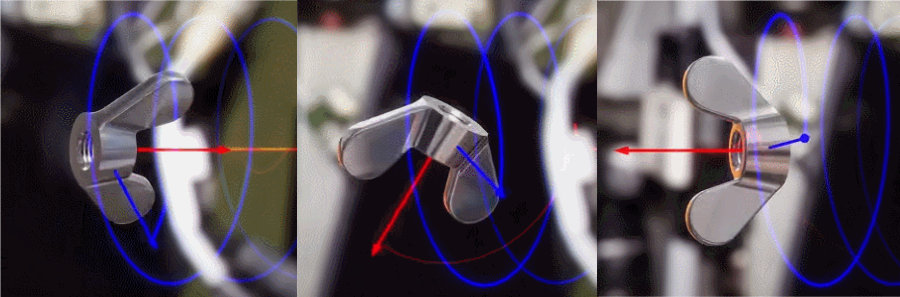
\includegraphics[width=0.9\textwidth]{dzhani.jpg}
\end{center}
   \caption{ພາບປະກອບຂອງຜົນກະທົບ Dzhanibekov \cite{28}.}
\label{fig:10}
\end{figure*}

ຫຼັກການທີ່ອະທິບາຍການປ່ຽນແປງຢ່າງໄວໃນແກນຫມຸນຂອງໂລກມີພື້ນຖານໃນຟິດສິກສ໌ຂອງວັດຖຸທີ່ກຳລັງຫມຸນ. ຕົວຢ່າງມາດຕະຖານຂອງນີ້ ແມ່ນຜົນກະທົບ Dzhanibekov ທີ່ພົບໂດຍນັກບິນອວກາດຊາວຣັດເຊຍ Vladimir Dzhanibekov \cite{37} ແລະຖືກສະແດງໃນຮູບທີ່ \ref{fig:10}. ວັດຖຸທີ່ບໍ່ໄດ້ຫມຸນຢ່າງສົມບູນໃນແກນອິນເນີເຊຍຫຼັກທັງສາມຂອງມັນ ຈະບໍ່ສາມາດຮັກສາແກນຫມຸນໄວ້ໄດ້ຢ່າງຄົງທີ່. ຖ້າມັນກຳລັງຫມຸນໃກ້ກັບແກນອິນເນີເຊຍທີ່ສອງ ມັນຈະເກີດປາກົດການປ່ຽນແປງຢ່າງກະທັນຫັນໃນການຫມຸນ. ເຖິງແມ່ນວ່ານີ້ຈະບໍ່ແມ່ນສິ່ງທີ່ເຮົາເຊື່ອວ່າເກີດຂຶ້ນໃນເວລາທີ່ໂລກປ່ຽນແປງແກນຢ່າງໄວ ແຕ່ຫຼັກການຄືວ່າ ໃນກໍລະນີທີ່ບໍ່ມີແຮງພາຍນອກ ແມ່ນຟິດສິກສ໌ການຫມຸນເທົ່ານັ້ນທີ່ອະທິບາຍການປ່ຽນແປງແກນຫມຸນຂອງໂລກໄດ້ຢ່າງຮວດເຮວ.

ເພື່ອໃຫ້ຖືກຕ້ອງ, ໂລກເກືອບຈະບໍ່ເຄີຍປະສົບທຽບຄຽງກັບຜົນກະທົບ Dzhanibekov ຢ່າງງ່າຍໆ ແລະສະເໝີ. ຖ້າມັນເປັນເຊິ່ງນັ້ນ ເຮົາຈະສາມາດກວດພົບການປ່ຽນແປງແກນຫມຸນຂອງໂລກເປັນຂະບວນການຕາມເວລາ. ແຕ່ເຮົາເຊື່ອວ່າໂລກປະສົບການລົບກວນຢ່າງກະທັນຫັນ ແລະເປັນຮອບໆໃນໂຄງສ້າງທາງຟິດສິກຂອງມັນ ເຮັດໃຫ້ແຍກກັນລະຫວ່າງ "ສ່ວນຫມຸນດ້ານນອກ" (ເກືອບ/ແມນເທິນ) ແລະ "ຮ່າງກາຍຫມຸນດ້ານໃນ" (ເຂົາໃນ). ບໍ່ມີການໃສ່ແຮງພາຍນອກ, ກົດໝາຍຂອງການຮັກສາປະລິມານ ມຸມຫມຸນລະບຸວ່າ ໂລກບໍ່ສາມາດປ່ຽນແກນຫມຸນໄດ້ຢ່າງກະທັນຫັນ, ຓະນັ້ນການແຍກກັນລະຫວ່າງຮ່າງກາຍຫມຸນດ້ານນອກແລະດ້ານໃນ ແມ່ນໃຫ້ເຫັນເຖິງສິ່ງຫນຶ່ງໃນບັນດາສິ່ງຈຳນວນນ້ອຍເທົ່ານັ້ນ, ນອກຈາກການປະທະຈາກພາຍນອກ, ທີ່ສາມາດເຮັດໃຫ້ເກີດການປ່ຽນແປງຢ່າງກະທັນຫັນແລະລວດເຮວໄດ້.

ຂະບວນການເຉົ້າໜ້າສະເພາະທີ່ສ້າງການລົບກວນພາຍໃນໂລກເຊື່ອວ່າ ເປັນການປ່ຽນສະພາບຂອງໂຄງສ້າງເຫຼັກທີ່ສ້າງເປັນເຂົາໃນຂອງໂລກ (ຮູບທີ່ \ref{fig:11}). ເຂົາໃນປະກອບດ້ວຍເຫຼັກຮູບແບບ hexagonal close-packed (Fe) \cite{141}. ເມື່ອ hcp-Fe ນີ້ຖືກປຽນໃປເປັນສະພາບເຫຼວທີ່ເປັນເຫຼັກ, ມັນຈະປ່ອຍພະລັງງານຈະລະເຄີນ ແລະຖືກກົງໄປສູ່ເຂົານອກ. ການປ່ຽນສະພາບນີ້ທຳໃຫ້ຄວາມສາມາດນຳເມເຫລັກຂອງເຂົາລົດລົງ, ອ່ອນແຮງສະໜາມເຫລັກໂລກ, ແລະປ່ອຍຄວາມຮ້ອນ ເຮັດໃຫ້ເກິດໂຄງສ້າງ LLVP (large low-velocity shear province) (ຮູບທີ່ \ref{fig:12}) \cite{38} ໃນແມນເທິນ, ແລະທຳໃຫ້ຜິວໂລກຮ້ອນຂຶ້ນຜ່ານມະຫາສະມຸດນໍ້າລຶກ. ທັງສອງແນວໂນ້ມນີ້ໄດ້ຖືກບັນທຶກໄວ້ຢ່າງດີໃນສັດຕະວັດທີ່ຜ່ານມາ ແລະຈະຖືກອະທິບາຍແລະວິເຄາະໃນສ່ວນຕໍ່ໆໄປຂອງບົດຄວາມນີ້.

\begin{figure*}[t]
\begin{center}
% \fbox{\rule{0pt}{2in} \rule{.9\linewidth}{0pt}}
\includegraphics[width=1\textwidth]{layers.jpg}
\end{center}

   \caption{ຮູບແບບຂອງຂະບວນການພາຍໃນໂລກທີ່ນຳໄປສູ່ການກັບທິດ ECDO \cite{129}.}
\label{fig:11}
\end{figure*}


\begin{figure}[t]
\begin{center}
% \fbox{\rule{0pt}{2in} \rule{0.9\linewidth}{0pt}}
   \includegraphics[width=1\linewidth]{llvp.jpg}
\end{center}
   \caption{ພາບລາຍລະອຽດຂອງ LLVP ທາງໃຕ້ອາຟຣິກາໃຕ້ \cite{28}.}
\label{fig:12}
\label{fig:onecol}
\end{figure}


ຂະບວນການນີ້ຊື່ງເກີດຂຶ້ນພາຍໃນໂລກແບບກັບທາງ ນອກຈາກນັ້ນຍັງເຊື່ອວ່າເປັນສາເຫດທີ່ນຳໄປສູ່ການປ່ຽນກັບສະຖານະການຫມຸນຂອງໂລກຍ່ອນເວລາຫຼັງຈາກການກັບທິດ.

\section{ຫຼັກຖານສຳລັບການກັບທິດຂອງໂລກ}
There is strong reason to believe that we are on the brink of another Earth flip. A cataclysm has not occurred for several millennia, which is approximately the frequency with which these events seem to happen based on historical accounts and data. The strongest data supporting an impending flip comes from recent geomagnetic data, which indicates that the Earth's geomagnetic field has been weakening for approximately two thousand years. This weakening has been accelerating and has reached alarming rates in the last few decades.

Depicted in Figure \ref{fig:14} is the geomagnetic field of Earth in 1590 and 2025 \cite{125,126}. As shown in the figure, the field has weakened significantly.

Another metric for the weakening geomagnetic field is the position of the geomagnetic north pole (Figure \ref{fig:13}). Geomagnetic north has historically been located in the Canadian Arctic. However, it has been wandering slowly over the last several centuries, and accelerated significantly a few decades ago. It is now moving rapidly towards Russia at a rate of 55 kilometers per year \cite{124}.

\begin{figure*}[t]
\begin{center}
% \fbox{\rule{0pt}{2in} \rule{.9\linewidth}{0pt}}
\includegraphics[width=0.9\textwidth]{saa.jpg}
\end{center}
   \caption{ພາບພິມພາບຂອງພາກເຫນືອຂອງສະໜາມສີຂອງພິມສັນຍາປືນຂອງໂລກຈາກປີ 1590 ຫາ 2025. ຄຳນວນໂດຍໃຊ້ແບບຈຳລອງ gufm1 ແລະ IGRF-14 \cite{125,126}.}
\label{fig:14}
\end{figure*}

\begin{figure}[t]
\begin{center}
% \fbox{\rule{0pt}{2in} \rule{1\linewidth}{0pt}}
   \includegraphics[width=1\linewidth]{npw.jpg}
\end{center}

```latex
   \caption{ຕຳແໜ່ງຂອງຂົງເໜືອມັງຫະນິຍົມຈາກປີ 1590 ຫາ 2025, ທີ່ຖືກສະແດງໃນລະຫວ່າງທຸກ 5 ປີ \cite{142}.}
\label{fig:13}
\label{fig:onecol}
\end{figure}

\begin{figure}[t]
\begin{center}
% \fbox{\rule{0pt}{2in} \rule{1\linewidth}{0pt}}
   \includegraphics[width=1\linewidth]{ocean-highlight.jpg}
\end{center}
   \caption{ອັດຕາການອຸ່ນຂອງມະຫາສະມຸດໃນຄວາມເລິກ ($>$2000 m) ຈາກປີ 1991 ຫາ 2010, ຖືກວົງໄວ້ດ້ວຍສີແດງ \cite{132}.}
\label{fig:15}
\label{fig:onecol}
\end{figure}

ມີຄວາມເຊື່ອວ່າສະໜາມເຫຼັກຂອງໂລກເກີດຈາກດິນໄຟພາຍໃນ—ເສົາກົມຂອງກະແສມະການທີ່ເຄື່ອນທີ່ໃນແກມໄພນອກຂອງໂລກເນື່ອງຈາກການຫມຸນຂອງມັນ \cite{123}. ການອ່ອນກຳລັງຂອງສະໜາມເຫຼັກມັງຫະນິຍົມເປັນອາການຂອງຄວາມບົກພ້ອງທີ່ເກີດລຶກໆພາຍໃນໂລກ. ຕາມທຶດສະດີ ECDO, ຄວາມບົກພ້ອງເຫຼົ່ານີ້ຈະຜະອອກຄວາມຮ້ອນ ແລະສຸດທ້າຍກໍໃຫ້ແກມແລະແກມໄພສູນຈາກກັນ, ເຮັດໃຫ້ໂລກກົງຫົວ \cite{1}.

ມີຂໍ້ມູນຫຼາຍຢືນຢັນການມີຢູ່ຂອງຂະບວນການພາຍໃນໂລກແບບປ່ອຍຄວາມຮ້ອນ. ໂລກທີ່ອຸ່ນຂຶ້ນປາກົດໃນອຸນຫະພູມພື້ນດິນແລະພື້ນຜິວມະຫາສະມຸດທີ່ເພີ່ມຂຶ້ນ \cite{127,128}, ລະດັບ CO2 ໃນອາກາດເພີ່ມຂຶ້ນແບບຄວບຄູ່ກັບເປັນກິດກັບສາຍຄວາມຮ້ອນຂອງໂລກ \cite{129,130}, ແລະການຫຼຸດລົງຂອງດອກນຳ້ແຂງໃນທົ່ວທຸກໂລກ \cite{131}. ຂໍ້ມູນບົວຊີ້ໃຫ້ເຫັນວ່າລະດັບ CO2 ແລະອຸນຫະພູມທີ່ເພີ່ມແມ່ນບໍ່ເປັນສາເຫດຂອງການປ່ຽນແປງສະພາບອາກາດ “ທີ່ມະນຸດເຮັດຂຶ້ນ” ແຕ່ເປັນຜົນຢູ່ພາຍຫຼັງຂອງແກນໂລກທີ່ປ່ອຍຄວາມຮ້ອນ \cite{129}.

ສ່ວນທີ່ສຳຄັນທີ່ສຸດ, ການສຶກສາອັດຕາຄວາມຮ້ອນໃນມະຫາສະມຸດລຶກ (ເພີ່ນຄວາມເລິກ $>$2000 ແມັດ) ຊີ້ໃຫ້ເຫັນວ່າບໍ່ພຽງແຕ່ມະຫາສະມຸດລຶກກຳລັງອຸ່ນຂຶ້ນ, ແຕ່ອັດຕາອຸ່ນທີ່ແຮງທີ່ສຸດພົບໃນຊັ້ນອາບິສ (4000 - 6000 m). ການອຸ່ນຂຶ້ນໃນທະເລລຶກນີ້ມີສູນກາງຢູ່ລຶກກ່ວາ 4000 ແມັດ \cite{132,129}, ຈະບໍ່ສາມາດເປັນໄດ້ຖ້າທະເລຖືກອຸ່ນຈາກຂ້າງເທິງໂດຍບັນຍາກາດ. ຂໍ້ມູນເຫຼົ່ານີ້ສົ່ງຜົນໃຫ້ແກ່ຄວາມເຊື່ອມໂຍງຢ້ອນວ່າການປ່ຽນແປງອາກາດລ່າສຸດແລະສະໜາມເຫຼັກມັງຫະນິຍົມແມ່ນເກີດຈາກຂະບວນການຢູ່ລຶກໆພາຍໃນໂລກ. ຮູບທີ່ \ref{fig:15} ສະແດງອັດຕາການອຸ່ນຂອງທະເລລຶກທົ່ວໂລກຈາກປີ 1991 ຫາ 2010 \cite{132}.
```
\section{ການສ້າງແບບຈຳລອງການກຳລັງຈະເກີດພາບ Earth ກັບດ້ານ}

\begin{figure}[b]
\begin{center}
% \fbox{\rule{0pt}{2in} \rule{1\linewidth}{0pt}}
   \includegraphics[width=1\linewidth]{saa-crop.jpeg}
\end{center}
   \caption{ການຄຳນວນຈຸດກັບດ້ານຕາມ South Atlantic Anomaly ຊີ້ໃຫ້ເຫັນວັນທີ 13 ມີນາ 2059 \cite{125,126}.}
\label{fig:16}
\label{fig:onecol}
\end{figure}

ການຄາດໄລເວລາການກັບດ້ານຕໍ່ໄປຂອງໂລກເປັນວຽກງານທີ່ສັບສົນ. ທ້າວເຮົາມີແບບຈຳລອງທີ່ດີທີ່ສຸດໃນຕອນນີ້ເທິງພື້ນຕິດຊັບໃນຟິວເຕັກເທົານະຈິງຂອງໂລກ - South Atlantic Anomaly (SAA). ພື້ນທີ່ນີ້ເຫື້ອນເທິງທະເລ South Atlantic ເຫັນວ່າມີຄ່າແຮງຟິວເຕັກເທົານະອ່ອນທີ່ສຸດ ແລະ ຖືກກຳນົດເຖິງເປັນພື້ນທີ່ທີ່ມີແຮງຟິວຕໍ່າກວ່າ 32,000 nanoteslas \cite{135}, ຊຶ່ງເປັນຄ່າຟິວອ່ອນທີ່ສຸດໃນປີ 1590. ພື້ນທີ່ South Atlantic Anomaly ໄດ້ເພີ່ມຢ່າງຫຼວງຕັ້ງແຕ່ 1\% ຂອງພື້ນຜິວໂລກໃນປີ 1590 ເຖິງ 21\% ໃນປີ 2025 \cite{136}.

ເພື່ອໄດ້ຄາດເວລາປະເມີນເມື່ອໃດໂລກອາດຈະກັບດ້ານ, ຂ້ອຍໄດ້ນຳຂໍ້ມູນພື້ນທີ່ SAA ໄປປັບແບບກັບສູດ power-law tipping point, ເຊິ່ງເປັນການແບບຈຳລອງລະບົບສັບສົນກໍ່ຈະເຖິງຈຸດຜ່ານແບບສຳຄັນ ເມື່ອລະບົບມີການປ່ຽນແປງຢ່າງເຫຼືອສາຍ ແລະ ກະທັນຫັນ. ການຄຳນວນຂອງຂ້ອຍໄດ້ວັນທີກັບດ້ານທີ່ຄາດໄວ້ຄື 13 ມີນາ 2059 (ຮູບ \ref{fig:16}). ການຄາດໄລນີ້ຈະຖືກຕ້ອງຂື້ນເຣື່ອຍໆເມື່ອເຮົາເຂົ້າໃກ້ກັບຈຸດຜ່ານ \cite{136}.

ຕົວຊີ້ວັດອື່ນໆ ເຊັ່ນ ການເປັນໄປຂອງແກນຫມຸນ, ພິບັດອາກາດ, ແລະ ຂໍ້ມູນເກົາະສັນແລະພູໄຟ ກໍ່ສາມາດຊ່ວຍໃຫ້ພວກເຮົາຄາດໄດ້ດີຂຶ້ນເມື່ອໂລກກັບດ້ານຄັ້ງຕໍ່ໄປອາດຈະເກີດ.

\section{ເວລາທີ່ຜ່ານມາຂອງ ECDO}
While establishing an exact timeline for past ECDO events is difficult, it seems that there were at least 2 ECDO events during the Holocene. ກະລຸນາສັງເກດບັນທຶກທີ່ Herodotus ໄດ້ຮຽນມາຈາກພະສົງອີຢິບ ທີ່, \textit{"ຈາກພຣະມະຫາກະສັດອົງທ້າຍໄປເຖິງພຣະສົງຂອງ Hephaistos ຜູ້ປົກຄອງຄົນສຸດທ້າຍ, ມີການຜ່ານມາຂອງພັນທະລະວົງມະນຸດສຳລັບສາມຮ້ອຍສີ່ສິບເອັດຊົນ... ທ້າຍນີ້ພວກເຂົາໄດ້ກ່າວວ່າ ຕາເວັນໄດ້ຍ້າຍຈາກທີ່ຂຶ້ນຕົ້ນມາສີ່ຄັ້ງ, ແລະທີ່ສວນທີ່ມັນລົງໄປໃນປັດຈຸບັນນັ້ນ, ຕາເວັນໄດ້ຂຶ້ນສອງຄັ້ງ, ແລະໃນສະຖານທີ່ທີ່ມັນຂຶ້ນໃນປັດຈຸບັນ ມັນກໍເຄີຍລົງສອງຄັ້ງ"} \cite{32}. Plato, ຜູ້ທີ່ມີຊີວິດໃນສະຕະວັດທີ່ຫ້າ ກ່ອນຄຣິດການ \cite{111}, ໄດ້ກ່າວວ່າຫຼັງນ້ຳຖ້ວມທີ່ໄດ້ທຳລາຍ Atlantis ໃນວັນເດີຍຄືນເດຽວ 9,000 ປີກ່ອນ, \textit{"ນັບແຕ່ນັ້ນມາມີນ້ຳຖ້ວມຫຼາຍຄັ້ງ, ແລະຜູ້ທີ່ຍັງມີຊີວິດຢູ່ໃນເຂົາທຳຜົນ ບໍ່ຮູ້ຈັກສິນສະຫມຸບ ແລະຕະຫຼອດພັນທະລະວົງສະເໝີເຮັດຫຍັງເພື່ອຫາຄືນສິ່ງທີ່ເຫັນດີ"} \cite{112}, ຊຶ່ງບົດບອກວ່າອາດຈະມີຫຼາຍກວ່າສອງຄັ້ງຕັ້ງແຕ່ໝົດສຸດຍຸກ Younger Dryas ປະມານ 9700 ກ່ອນຄຣິດການ. ພະຍານຫຼັກທາງກາຍະພາບທີ່ກ່າວເຖິງໃນເອກະສານນີ້ ແລະໃນຜົນງານຄົ້ນຄວ້າຂອງຂ້ອຍ \cite{2} ໃຫ້ຫຼັກຐານຫນາແນ້ນເພື່ອຊີ້ຫົວໃຈເລື່ອງ Plato.

The most recent candidate date for an ECDO flip is during the period of 2300 to 1600 BCE, to which many cataclysmic flood accounts (Gun-Yu \cite{113,114,115}, Ogyges \cite{116,117}, Peru \cite{118,119}, Exodus \cite{120}), civilizational destructions and abandonments (Mohenjo-Daro \cite{121}, Minoan Crete\cite{100,101}) ແລະຄວາມພິລຶກທາງກາຍະພາບ (bond events \cite{122}, 4.2 kiloyear event \cite{90}) ຖືກກໍານົດວັນທີ່. ບໍ່ມີຫຼັກຐານໃດໜາແນ້ນກວ່ານີ້ທີ່ບົດບອກເຖິງເຫດການຄວາມຫຼວງຫຼາຍເຫດການໃຫຍ່.

\section{Conclusion}

Operation NANOOK ແມ່ນການປະຕິບັດງານລະດັບສົງຄາມເຢັນຂອງສະຫະລັດທີ່ມຸ່ງສໍາຫຼວດແຜ່ນທີ່ Arctic ແລະຊາຍຝັ່ງສົວເວັດທາງເໜືອຫຼັງສົງຄາມໂລກຄັ້ງທີ II \cite{137}. ໃນລະຫວ່າງການສືບສວນຂອງພວກເຂົາ, ພວກເຂົາໄດ້ພົບວ່າແກນແມ່ເຫຼັກຢູ່ຫ່າງຈາກຈຸດທີ່ຄວນຢູ່ຕາມຜົນການສຳຫຼວດເກົ່າ 125 ຫາ 200 ໄມລ໌. ນຳພາຍ, \textit{"ໃນກຸ່ມນັກວິທະຍາສາດຂອງລັດ, ເກີດຄໍາຖາມວ່າຈະເປັນແນວໃດເມື່ອແກນແມ່ເຫຼັກແລະແກນພູມິສາດສົງບັນຈົບ. ເພື່ອຫາຄໍາຕອບ, ພາຍໃຕ້ການຄຸ້ມຄອງຂອງ Dr. Paul A. Siple, Rand Corporation ໄດ້ຖືກວ່າຈ້າງເພື່ອສຶກສາໃນຫ້ອງປຏິບັດ ໂດຍສ້າງແບບຈຳລອງຂອງໂລກເປັນຊັ້ນຊັ້ນ – ໂລກວົງໃນເປັນໂລຫະໄຟຟ້າທີ່ໝຸນຢູ່ກັບແກນຜູ້ກຳນົດ “ແມ່ເຫຼັກ”; ແລະວົງນອກເປັນແກນພູມິສາດທີ່ໝຸນເປັນ “ຂັ້ນຂອງໂລກ” ງານສຶກສາຢຶງຢືນດ້ວຍການທົດລອງຊໍ້າໆ ວ່າເມື່ອ “ແມ່ເຫຼັກ” ເຂົ້າໄປໃກ້ “ພູມິສາດ”, “ແມ່ເຫຼັກ” ຈະເລີ່ນຄວາມໄວເສື້ອກັບພູມິສາດ, ແລະຈະກະໂດດປະສານກັນ; ແຕ່ແທນທີ່ແກນຈະປະສານ, “ແມ່ເຫຼັກ” ຈະ “ກັບທິດ” ຫຼຽວໄປຮອບ “ພູມິສາດ” ແລ້ວເຄື່ອນອອກໄປທາງເສັ້ນສູນສຸມ ມາຢູ່ຕໍາແໜ່ງທີ່ແກນທັງສອງມີມຸມຊອງ 89 ອົງສາ. ຫຼັງຈາກ “ກັບທິດ” ຫຼັງນີ້, ແກນທັງຫມົດຈະວົບມາຮ່ວມກັນແບບຊ້າໆ ຕາມການຜ່ານໄປຂອງເວລາ"} \cite{138,139}.

ຕໍ່ມາເທົ່ານັ້ນ, \textit{"ໃນການປະຊຸມທາງວິທະຍາສາດເທື່ອໜຶ່ງທີ່ Major White ເຂົ້າຮ່ວມໃນ Pentagon ຕົ້ນປີ 1948, ນັກວິທະຍາສາດໄດ້ອະທິບາຍເຖິງຄວາມເໝາະສົມໃນການແຈ້ງຕົວປະຊາຊົນເຖິງປະກົດການກັບແກນຂອງໂລກ. ບໍ່ອະນຸມັດໃຫ້ປິດບັງຂໍ້ມູນຈາກປະຊາຊົນ; ແຕ່ຫຼາຍຄົນບໍ່ສາມາດຕົກລົງກັນໄດ້ວ່າຈະເຜີຍແພ່ແນວໃດ. ຄວາມຮູ້ເຫຼົ່ານີ້, ໃນຄວາມຮູ້ສຶກຂອງບາງຄົນ, ສາມາດທຳລາຍຈິດສຳນึกໃນສັງຄົມເອງ. ຄວາມກັງວົນນີ້ບໍ່ເຫັນຈິງເມື່ອປະມານປີ 1950, ຂໍ້ມູນກ່ຽວກັບປະກົດການກັບແກນໄດ້ຖືກເຜີຍແພ່ຜ່ານຫົວຂໍ້ຂ່າວແລະວາລະສານ, ແຕ່ນ່າແປກໃຈບໍ່ມີປະຊາຊົນຕອບຮັບ ເຫມືອນຖືກເອື້ອສານປະຫວັດສາດແບບພື້ນເມືອງ ຫຼືບໍ່ເຊື່ອ"} \cite{138,139}.

ເຫດໃດພວກເຮົາບໍ່ເອົາໃຈໃສ່ຕໍ່ນີ້? ມີເຫດຜົນຫຼາຍທີ່ເຮັດໃຫ້ເຊື່ອວ່າໂລກເຄີຍກັບທິດມາແລ້ວ. ເອກະສານນີ້ ພ້ອມດ້ວຍພາກສອງ ອະທິບາຍຫຍໍ້ຍ່ອດຫຼັກຐານຫຼາຍສາຂາມາຮ່ວມກັນທີ່ສະແດງວ່າມັນເປັນແນວນັ້ນ, ເຊັ່ນ ເລື່ອງນ້ຳຖ້ວມທົ່ວໂລກ, ຊິ້ນດິນແລະຊີວິດທະເລປົກດິນມີຢູ່ທົ່ວບົດບົນ, ທີ່ຢູ່ພະຍາບານໃຕ້ດິນເກົ່າແກ່, ຊິ້ນສ່ວນສັດ, ແລະພູດິນຫຼວງເຊັ່ນນັ້ນ. ມະນຸດເກົ່າວ່າເປັນແສນໆປີ ແຕ່ປະຫວັດສາດສະໄໝໃໝ່ມີພຽງບໍ່ກີ່ພັນປີ. ເປັນໄປໄດ້ບໍ່ວ່າທຸກຄັ້ງທີ່ເວລາໜຶ່ງໂລກກັບທິດ ທະວີປີ້ຫຼົ້ມຖືບ ແລະພວກເຮົາຕ້ອງກັບໄປຈຸດເລີ່ມຕົ້ນ - ຍຸກຫີນ - ທຳໃຫ້ບັນທຶກປະຫວັດສາດກ່ຽວກັບສະໄໝເກົ່າເຫຼືອເປັນພຽງຫຍັງເລື່ອງນ້ຳຖ້ວມຫຼວງເທົ່ານັ້ນ? ຖ້າໃຊ້ແລ້ວ, ການປ້ອງກັນເຫດການນີ້ແມ່ນໜ້າວຽກທີ່ສຳຄັນທີ່ສຸດອັນໜຶ່ງຂອງມະນຸດຊາດ.

ຕົວຢ່າງດອກໄມ້ທີ່ຂ້ອຍຍົກໃນທ້າຍນີ້ມາຈາກ Timaeus ເປັນການສົນທະນາລະຫວ່າງໂຊລອນ ນັກການເມືອງອະເທນ ແລະພະສົງອີຢິບ \cite{140} : \textit{"ໃນຄັ້ງໜຶ່ງ, ເມື່ອ [ໂຊລອນ] ຕ້ອງການນໍາເອົາເຣື່ອງປະຫວັດສາດມາສົນທະນາ ເຂົາໄດ້ເພີ່ມເລື່ອງລາວເກົ່າທີ່ສຸດຂອງເຮົາ, ເກັ່ງກາຍ Phoroneus ຜູ້ເກັ່ງກາຍເທົ່າທີ່ຖືກເວົ້າວ່າເປັນມະນຸດອົງທ້າຍ, ແລະ Niobe; ເຂົາຍັງໄດ້ຕໍ່ດ້ວຍເລື່ອງ Deucalion ແລະ Pyrrha ຫຼັງນ້ຳຖ້ວມ ແລະການລອດຊີວິດ ແລະບອກຮາກພັນທະລະວົງ ເມື່ອນັບຈໍານວນປີຂອງເຫດການແຕ່ລະໃນນັ້ນໃສ່, ເພື່ອ ຄຳນວນເທົ່າໄຫລ່ສະໝັກເວລາ. ພະສົງແກ່ຄົນໜຶ່ງໄດ້ເວົ້າວ່າ “ໂຊລອນ, ໂຊລອນ, ຊາວກຣີກເຈົ້າເປັນແດ່ວຍເດັກນ້ອຍເທື່ອ ບໍ່ມີຊາວກຣີກເກົ່າເຕັມທີ່.” ເມື່ອໄດ້ຟັງນີ້ເຂົາຖາມຢ່າງໄດ້ວ່າ “ປະໂຫຍກນີ້ໝາຍຄວາມວ່າແນວໃດ?” ແລະພະສົງກໍໄດ້ຕອບວ່າ “ພວກເຈົ້າເດັກນ້ອຍທີ່ຈິດໃຈ, ທຸກຄົນ. ພວກເຈົ້າບໍ່ມີແນວຄິດທີ່ສືບເນື່ອງຈາກປະພັນທຳ ແລະບໍ່ມີວິທະຍາສາດອັນເກົ່າ. ມີການທຳລາຍມະນຸດຊາດຫຼາຍຄັ້ງ, ເຊັ່ນ ໄຟ ແລະນ້ຳ, ແລະການຖືກທຳລາຍດ້ວຍສາເຫດອື່ນ. ເລື່ອງທີ່ເຂົາລ່າວໃນດິນແດນພວກເຈົ້າແລະເຮົາ, ເຊັ່ນ ເທື່ອ Phaethon, ລູກ Helios ໄດ້ຂຶ້ນຂີ່ລົດບິນຂອງພໍ່, ແຕ່ບໍ່ສາມາດຂັບໄດ້ ເລີຍເຜົາທຸກສິ່ງບນໂລກແລະຕົນເອງ, ນັ້ນເປັນເພີງເທິງປະຫວັດສາດ ແຕ່​ຄວາມ​ຈິງ​ແມ່ນ​ໃນ​ການ​ເກີດ​ຂອງ​ການ​ເຄື່ອນ​ຂອງ​ດາວ​ເຄື່ອນ​ຮອບ​ໂລກ​ແລະ​ການ​ຖືກ​ທຳລາຍ​ເທິງ​ໂລກ​ໂດຍ​​ໄຟ​ຕ່າງ​ໆ, ຊຶ່ງເກີດຂຶ້ນເປັນຮອບ. ເທື່ອນັ້ນຜູ້ຢູ່ເຂົາຮາບເໜືອມັກຖືກທຳລາຍມາກກວ່າຜູ້ຢູ່ແພດນ້ຳ, ແລະໃນກໍລະນີຂອງພວກເຮົາ ແມ່ນ Nile ຜູ້ອຸປະຖຳ⚶ນະນົວທີ່ອື່ນທີ່ຊ່ວຍທຳລາຍນີ້. ແຕ່ເມື່ອພຣະເຈົ້າຖັກທໍາແຜ່ນດິນດ້ວຍນ້ຳ, ຄົນເລີ້ຍສັດຢູ່ເຂົາໄດ້ລອດຊີວິດ, ແຕ່ຄົນໃນເມືອງເຈົ້າຈົນເປັນອັນຕາລາຍ, ຂອງພວກເຮົານ້ຳເປັນແຕ່ໄຫຼຈາກຂ້າງລຸ່ມ. ສະນັ້ນຄວາມຈິງທີ່ບັນທຶກນີ້ຢູ່ນີ້ແມ່ນເກົ່າເກັບໄວ້ຫຼາຍທີ່ສຸດ; ຊື່ງແມ່ນທຸກເສັ້ນທາງຜ່ານທີ່ບໍ່ຮ້ອນຫຼືໜາວເກິນໄປ ຈະມີມະນຸດຢູ່ເສມອະທິບາຍຫຼາຍຫຼືນ້ອຍ. ແລະຖ້າເກີດເຫດການໃດທີ່ສຳຄັນ ຫຼືນ່າສົນໃຈໄວ້ແມື່ນໃນປະເທດເຈົ້າ ຫຼືພວກເຮົາ ຫຼືບ່ອນອື່ນ ທຸກເຫດການໄດ້ຖືກບັນທຶກໄວ້ໃນວັດວາອາລາມ; ໃນຂະນະທີ່ພວກເຈົ້າແລະອື່ນໆແມ່ນແຕ່ທຸກຄັ້ງໄດ້ຮັບອັກສອນ ແລະອາທິບາຍສິນທິບັງກັບໄປໃນຄືນ. ກວ່າປີໃດ, ຖ້ານ້ຳຖ້ວມຜ່ານມາ, ນັກຄົ້ນໄດ້ເຫັນແຕ່ຄົນບໍ່ຮູ້ອັກສອນ, ເຮັດໃຫ້ເຈົ້າເປັນເດັກນ້ອຍຕະຫຼອດ, ໂດຍບໍ່ຮູ້ເຄື່ອງວິຊາການອະດີດໃດເລີຍ. ຊັດເຈນເຫມືອນຢ່າງທີ່ເຈົ້າກ່າວເມື່ອກີ້ນີ້, ໂຊລອນ, ກ່ຽວກັບປະຊາຊົນຂອງເຈົ້າ, ເປັນເພີງເລື່ອງເດັກນ້ອຍ; ເພາະເຈົ້າຈື່ງຈືດີນ້ຳຖ້ວມເມື່ອງດຽວ, ແມ່ນອັນດຽວ, ທັງໆທີ່ສະເໝີມີຫຼາຍໆຄັ້ງກ່ອນນັ້ນ; ແລະຍັງບໍ່ຮູ້ຈັກເຫມືອນພວກສຸດທ້າຍທີ່ດີທີ່ສຸດໃນມະນຸດເກີດທີ່ດິນແດນເຈົ້າ ແລະເຈົ້າແລະເມືອງເຈົ້າກໍມາຈາກນັ້ນ, ແທ່ນກາງໄວ້ພຽງເຫຼືອເໝົາ. ແຕ່ນີ້ເຄິ່ງຂາດເພາະພັນທະລະວົງຫຼາຍຮຸ່ນບໍ່ສາມາດບັນທຶກຊື່. ເຄື່ອນໜຶ່ງເທື່ອເດີມກ່ອນນ້ຳຖ້ວມໃຫຍ່, ອາລະບອດອາເທນໄດ້ເປັນລັດສະໜາມທີ່ກ້າຫານແລະຈັດລະເບຽບທີ່ສຸດ. ເວົ້າວ່າໃນນັ້ນມີສິນລະປະອັນຫຼາຍແລະການປົກຄອງອັນດີ"}.

ພະສົງເຫຼົ່ານີ້ແນ່ນອນຍັງໄດ້ບອກເຖິງ Atlantis ເປັນຍ້ອນວ່າ: \textit{"ເພາະທຸກສິ່ງທີ່ຢູ່ນີ້ ຢູ່ໃນຮ່ອງທີ່ເຮົາເວົ້າຖຶ່ງ, ນັ້ນແມ່ນມີທາງເຂົ້າແຄບໆ; ແຕ່ອີກຟາກໜຶ່ງນັ້ນແມ່ນທະເລທີ່ແທ້ ແລະດິນອອມລອບມັນຄວນຮຽກວ່າທວົດທີ່ເປັນຈິງງາມ. ໃນເກາະ Atlantis ເທື່ອໜຶ່ງມີກໍລະປົກຄອງບາງຢ່າງ ແລະອຳນາດທີ່ຍິ່ງໃຫຍ່ທີ່ປົກຄອງເກາະດຽວ, ແລະຫຼາຍເກາະອື່ນກະທັ່ງບຶງພຣະຊະນະບົດບຸນ; ແລະ, ພາຍໃນຕອນນັ້ນເຂົາປົກຄອງດິນດອນອີກຫຼາຍໆສ່ວນດ້ວຍ; ແລະ, ຂອງດິນເຊິ່ງເວົ້າວ່າໄດ້ອອກຈາກ Straits, ພວກເຂົາປົກຄອງ Libya ຕໍ່ໄປຈາກ Egypt, ແລະຢູ່ເຖິງ Europe ຕໍ່ໄປ Tyrrhenia. ພວກນີ້ໄດ້ລວມຕົວກັນ, ຫາຍຄົນພິຈາລະນາປົກຄອງສັງຄົມເຮົາແລະເຈົ້າໃຫ້ເປັນອັນດຽວ, ຄວາມກ້າຫານຂອງເມືອງເຈົ້າໄດ້ກາຍເຫັນໃນສາຍຕາທົ່ວໄປ. ຫຼັງນັ້ນເກີດເຫດເຕືອນໃຈຄືແຜ່ນດິນໄຫວ ແລະນ້ຳຖ້ວມຫຼວງ, ແລະວັນຄືນອັນໃຫຍ່ເກີດຂຶ້ນ, ເມື່ອທະຫານເຮົາຖືກດິນກົກ, ແລະເກາະ Atlantis ກໍ່ຖືກທະເລດູດຫາຍ"}.

\section{Acknowledgments}

ຂອບໃຈ Ethical Skeptic, ຜູ້ຂຽນຕົ້ນສະບັບຂອງວິທະຍານິພົນ ECDO, ທີ່ໄດ້ສົ່ງຕໍ່ວິທະຍານິພົນທີ່ຫຼວງໃຫຍ່ຂອງຕົນແລະແບ່ງປັນໃຫ້ໂລກ. ວິທະຍານິພົນສາມພາກຂອງພວກເຂົາ \cite{1} ຍັງເປັນຄຳຂວັນຕັ້ງໃນເທດສະດີ ECDO (Exothermic Core-Mantle Decoupling Dzhanibekov Oscillation), ແລະມີຂໍ້ມູນຫຼາຍກວ່າທີ່ຂ້ອຍສະຫຼຸບແບບຫຍໍ້ໃນນີ້.
Thanks to Ankit, ຜູ້ທີ່ໄດ້ປະມວນຂໍ້ມູນການລວມຕົວ cataclysm ໃນຕາຕະລາງ 1.

ແລະແນ່ນອນ, ຂອບໃຈຕໍ່ບັນດາຍັກທີ່ພວກເຮົາຢືນຢູ່ເທິງໄຫລ່ຂອງພວກເຂົາ; ຜູ້ທີ່ໄດ້ເຮັດການຄົ້ນຄວ້າ ແລະ ການສືບສວນທັງໝົດທີ່ເຮັດໃຫ້ຜົນງານນີ້ເກີດຂຶ້ນໄດ້ ແລະ ເຮັດໃຫ້ແສງສວ່າງແກ່ມວນມະນຸດ.

\clearpage
\twocolumn

\section{ຮູບເພີ່ມເຕີມ}


\begin{figure}[H]
\begin{center}
% \fbox{\rule{0pt}{2in} \rule{1\linewidth}{0pt}}
   \includegraphics[width=1\linewidth]{wave.jpg}
\end{center}
   \caption{ການສັ່ງເກັບດູຢ່າງໃກ້ຊິດຕໍ່ຢ່າງ undercut, ການກັດເຊາແບບພາລາໂບລິກຂອງຄິວພິຣາມິດ Khafre \cite{27}.}
\label{fig:19}
\label{fig:onecol}
\end{figure}
\begin{figure}[H]
\begin{center}
% \fbox{\rule{0pt}{2in} \rule{1\linewidth}{0pt}}
   \includegraphics[width=1\linewidth]{star-stone.jpg}
\end{center}
   \caption{ແຜນທີ່ດາວທີ່ຖືກແກະສະຫວ່າງໃນຫິນຢູ່ໃນຫໍ່ໜຶ່ງຂອງພິຣາມິດ Khufu \cite{28}.}
\label{fig:20}
\label{fig:onecol}
\end{figure}

\begin{figure*}[t]
\begin{center}
% \fbox{\rule{0pt}{2in} \rule{.9\linewidth}{0pt}}
\includegraphics[width=1\textwidth]{deepsea.jpg}
\end{center}
   \caption{ພາບທັດລັກຂອງຄວາມຜິດປົກກະຕິການຮ້ອນໃນມະຫາສະມຸດລຶກແລະອາບິສຊາລທີ່ເທັບກັບຄວາມຮ້ອນຕາມປົກກະຕິຂອງອາກາດ-ມະຫາສະມຸດ. ຄວາມຜິດປົກກະຕິການຮ້ອນໂດຍລວມໄດ້ຖືກຢືມມາຈາກ NOAA \cite{147}, ການແບ່ງປັນຄວາມຮ້ອນຂອງມະຫາສະມຸດລຶກແລະອາບິສຊາລມາຈາກບົດສຶກສາຂອງ Desbruyeres \cite{132}, ແລະການປະມວນຜົນຂໍ້ມູນ ແລະ ການສະແດງຜົນໂດຍ Ethical Skeptic \cite{129}.}
\label{fig:21}
\end{figure*}
\begin{figure*}[t]
\begin{center}
% \fbox{\rule{0pt}{2in} \rule{.9\linewidth}{0pt}}
\includegraphics[width=1\textwidth]{sealevel.jpeg}
\end{center}
   \caption{ລະດັບນ້ໍາທະເລສະແດງໃຫ້ເຫັນການເພີ່ມຂຶ້ນ 20\% ຂອງຄວາມແປຜັນໃນໄລຍະເວລາ 75 ປີ ທົ່ວ 63 ສະຖານີ, ບົກບອກວ່າມີການເພີ່ມຄວາມໄວຂອງນໍ້າໄຫຼ. ການຫຼຸດພຸ່ງຂຶ້ນຂອງຄວາມແປຜັນນ້ໍາທະເລກຽວໃນຄາບຢູ່ກັບການເພີ່ມຂຶ້ນອຸນຫະພູມອ່າວທະເລ, ບົກບອກວ່າທັງສອງຢ່າງນີ້ອາດຈະເກີດຈາກຄວາມຮ້ອນທີ່ເກີດຈາກທາງໃຕ້ລຶກຂອງສະຫມຸດໂລກ \cite{2,129}.}
\label{fig:22}
\end{figure*}

\begin{figure*}[t]
\begin{center}
% \fbox{\rule{0pt}{2in} \rule{.9\linewidth}{0pt}}
\includegraphics[width=1\textwidth]{co2.jpg}
\end{center}
   \caption{ຄ່າ CO2 ໃນບະຫາກາດຕໍ່ລ້ານສ່ວນໄດ້ເພີ່ມຂຶ້ນຢ່າງຕໍ່ເນື່ອງຕະຫຼອດ 45 ປີຜ່ານມາ, ອາດເກີດຈາກການເພີ່ມຂຶ້ນຂອງອຸນຫະພູມທະເລ. ທີ່ມາ: NOAA \cite{148,129}.}
\label{fig:23}
\end{figure*}

\begin{figure*}[t]
\begin{center}
% \fbox{\rule{0pt}{2in} \rule{.9\linewidth}{0pt}}
\includegraphics[width=1\textwidth]{ice.jpg}
\end{center}
   \caption{ພື້ນທີ່ນໍ້າກ້ອນແຫ່ງໂລກໄດ້ຫຼຸດລົງຕະຫຼອດ 45 ປີຜ່ານມາ ເນື່ອງຈາກໂລກອຸ່ນຂຶ້ນ. ແຫຼ່ງຂໍ້ມູນ: ADS \cite{149}.}
\label{fig:24}
\end{figure*}

\clearpage
\twocolumn

{\small
\renewcommand{\refname}{ບັນຊີອ້າງອິງ}
\bibliographystyle{ieee}
\bibliography{egbib}
}

\end{document}